
\documentclass[a4paper,fleqn]{cas-sc}

\usepackage[authoryear]{natbib}
\chardef\bmmax=0
\chardef\hmmax=0
\usepackage{bm,tikz,enumitem,threeparttable,xcolor}
\usetikzlibrary{arrows.meta,positioning,fit}
\hypersetup{colorlinks=true,linkcolor=black,citecolor=black,urlcolor=blue}
\ExplSyntaxOn
\bool_gset_true:N \g_stm_nologo_bool
\ExplSyntaxOff
\newcommand{\R}{\mathbb{R}}
\newcommand{\B}{\mathcal{B}}
\newcommand{\V}{\mathcal{V}}
\newcommand{\I}{\mathcal{I}}
\newcommand{\softmax}{\operatorname{softmax}}
\newcommand{\IoU}{\operatorname{IoU}}
\newcommand{\mIoU}{\operatorname{mIoU}}
\newcommand{\temp}[1]{\textcolor{blue!65!black}{#1\textsuperscript{\ensuremath{\dagger}}}}
\begin{document}
\let\WriteBookmarks\relax
\def\floatpagepagefraction{1}
\def\textpagefraction{.001}
\shorttitle{AgriOcc}
\shortauthors{He, Jin and Liu}
\title[mode=title]{AgriOcc: Crop-Aware 3D Semantic Occupancy Prediction for Agricultural Mobile Platforms}
\author[1]{Lei He}
\author[1]{Jing Jin}[orcid=0000-0001-7753-7656]
\cormark[1]
\ead{jinjinghit@hit.edu.cn}
\author[2]{Yi Liu}
\affiliation[1]{organization={School of Astronautics, Harbin Institute of Technology},
 city={Harbin},postcode={150001},country={China}}
\affiliation[2]{organization={Zhengzhou Advanced Research Institute of Harbin Institute of Technology},
 city={Zhengzhou},postcode={450000},country={China}}

\begin{abstract}
Agricultural mobile platforms need to understand the 3D spatial relationships among crops, soil, drivable areas, and obstacles, whereas 2D crop-row detection and image segmentation cannot directly provide a unified spatial representation.
We propose AgriOcc, which predicts six-class semantic occupancy over a $15\times15\times5\,\mathrm{m}$ region in front of the mobile platform from forward, forward-left, and forward-right RGB images.
To address the anisotropy of plant and ground structures and the uneven distribution of crop supervision across agricultural scenes and samples, AgriOcc retains BEVFormer's deformable self-attention backbone and introduces an Agricultural Structure-Adaptive Mixture-of-Experts decoder (Agri-AMoE).
The decoder lifts BEV representations into a 3D feature volume, enhances the features with channel attention, and then uses spatial saliency and gradient energy to adaptively route among experts for local planar details, vertical structures, and broader context.
We also propose a crop-aware sampling strategy that replaces a small quota of training samples to increase exposure to samples containing crops, improving crop perception without increasing the amount of training data.
To address the scarcity and high acquisition cost of agricultural semantic occupancy data, we develop an Unreal Engine 5-based pipeline for constructing simulated agricultural scenes and build AgriOcc-Dataset, a synthetic 3D semantic occupancy dataset.
On this dataset, AgriOcc achieves 64.08\% mIoU and 39.38\% crop IoU, substantially outperforming other state-of-the-art 3D semantic occupancy methods.
AgriOcc also delivers substantial performance gains on the real-world off-road dataset ORAD-3D. In addition, crop-row fitting experiments using the 3D semantic maps predicted by AgriOcc demonstrate its practical utility in agricultural scenes.
Extensive experiments demonstrate AgriOcc's capabilities in agricultural scene understanding and transfer to real environments, offering an approach to 3D visual navigation for agricultural mobile platforms that balances accuracy and training cost.

\end{abstract}
\begin{keywords}
Agriculture \sep 3D semantic occupancy \sep mixture of experts \sep crop-aware sampling
\end{keywords}
\maketitle
\section{Introduction}\label{sec:intro}
Agricultural mobile platforms performing field inspection, crop protection, harvest transport, and autonomous navigation need to understand the spatial relationships among crops, furrows, soil, drivable areas, and unexpected obstacles. Existing visual navigation systems typically use a modular pipeline: crop-row recognition and road or drivable-area segmentation first produce 2D results, which are converted into navigation constraints through geometric fitting, coordinate transformation, and rule-based post-processing~\citep{nkwochaComprehensiveReviewSensing2025,baiVisionbasedNavigationGuidance2023}.
This pipeline has several limitations. First, 2D perception, geometric recovery, and transformation into the control coordinate frame are separate stages, allowing errors to accumulate. Second, 2D perception paradigms often require additional LiDAR or depth cameras to measure distances and estimate object poses. For obstacles of varying sizes and pedestrians on farms, 2D pixel-level results also have difficulty representing height and occluded space. Third, systems based on 2D perception often require multiple perception models to work together, introducing additional training and tuning costs.

3D semantic occupancy prediction represents the environment in a regular voxel grid in the mobile platform coordinate frame, assigning a semantic category to each voxel.
First, it provides free space, ground, crops, and obstacles through a unified interface for subsequent traversability analysis, collision checking, and visual navigation.
Second, it directly outputs a structured spatial representation without post-processing such as projection, filtering, or rasterization, providing better spatial consistency across cameras.
In addition, surrounding semantic information can support predictions in occluded regions, whereas depth maps predict only the nearest occupied point along each ray and cannot recover occluded parts of a 3D scene.
Compared with 2D semantic maps, occupancy representations explicitly preserve object height and spatial adjacency, providing a shared environmental description for subsequent traversability assessment, collision checking, and path planning.
Autonomous-driving research has shown that explicit lifting methods such as Lift--Splat--Shoot~\citep{philion2020lift,huang2021bevdet,li2022bevdepth}, as well as query-based methods such as DETR3D, PETR, and BEVFormer~\citep{wang2022detr3d,li2022petr,li2022bevformer}, can learn geometrically consistent bird's-eye-view representations from multi-camera images. These representations can further support dense occupancy~\citep{wei2023surroundocc,wang2023openoccupancy}, temporal scene prediction, and planning~\citep{zheng2024occworld,mei2025irwm}.
These methods commonly assume six surround-view cameras, omnidirectional road-traffic scenes, relatively large spatiotemporal ranges, and large models. Agricultural mobile platforms, in contrast, typically use controllers with limited computing capacity and operate in relatively static fields with forward-facing tasks.
We therefore focus on the most common forward field of view of agricultural mobile platforms during field operations: images from forward, forward-left, and forward-right cameras are used to predict 3D semantic occupancy over the $15\,$m region ahead.

However, directly transferring 3D semantic occupancy methods to agricultural tasks presents three key challenges.
First, farmland has distinctly directional spatial structures: the ground and crop rows extend horizontally, while canopies, stems, and obstacles have different vertical forms. If each BEV cell independently uses an MLP to predict classes at all heights, boundaries between neighboring plants and the ground tend to become blurred.
Second, the abundance of free space and background ground leads to substantial differences in the amount of crop supervision provided by individual samples. Simply increasing the crop loss weight does not increase effective crop observations, and excessive reweighting may also increase crop false positives.
Finally, real agricultural data are constrained by seasons, crop growth stages, field variation, sensor configurations, and annotation costs, making systematic studies across diverse field conditions difficult. Existing studies also often focus on a single crop, limiting research on generalization across regions and crop types.

To address these challenges, we first develop an Unreal Engine 5-based pipeline for constructing simulated agricultural scenes and build AgriOcc-Dataset, a synthetic 3D semantic occupancy dataset. It contains 298 complete sequences and 38,862 multi-view samples covering 10 crops, 3 growth stages, 5 times of day, and two weather conditions.
We then propose AgriOcc, a 3D semantic occupancy network for agricultural mobile platforms. As shown in Fig.~\ref{fig:overview}, ResNet--FPN first extracts multi-scale image features, and a BEVFormer-style encoder builds a unified BEV representation through deformable self-attention and spatial cross-attention to image features. We retain the current-frame deformable spatial aggregation capability of the original Temporal Self-Attention (TSA) module.
We introduce the Agricultural Structure-Adaptive Mixture-of-Experts decoder, Agri-AMoE, which lifts BEV features into a 3D feature volume and combines three anisotropic experts according to local gradient energy and spatial saliency to predict six-class occupancy.
In addition, we propose a training-time crop-aware sampling strategy that counts crop voxels within the current prediction region and replaces a small quota of samples to increase exposure to samples containing crops. This strategy substantially improves crop perception without increasing the number of samples per epoch or changing the inference network.

\begin{figure}[pos=htbp]
\centering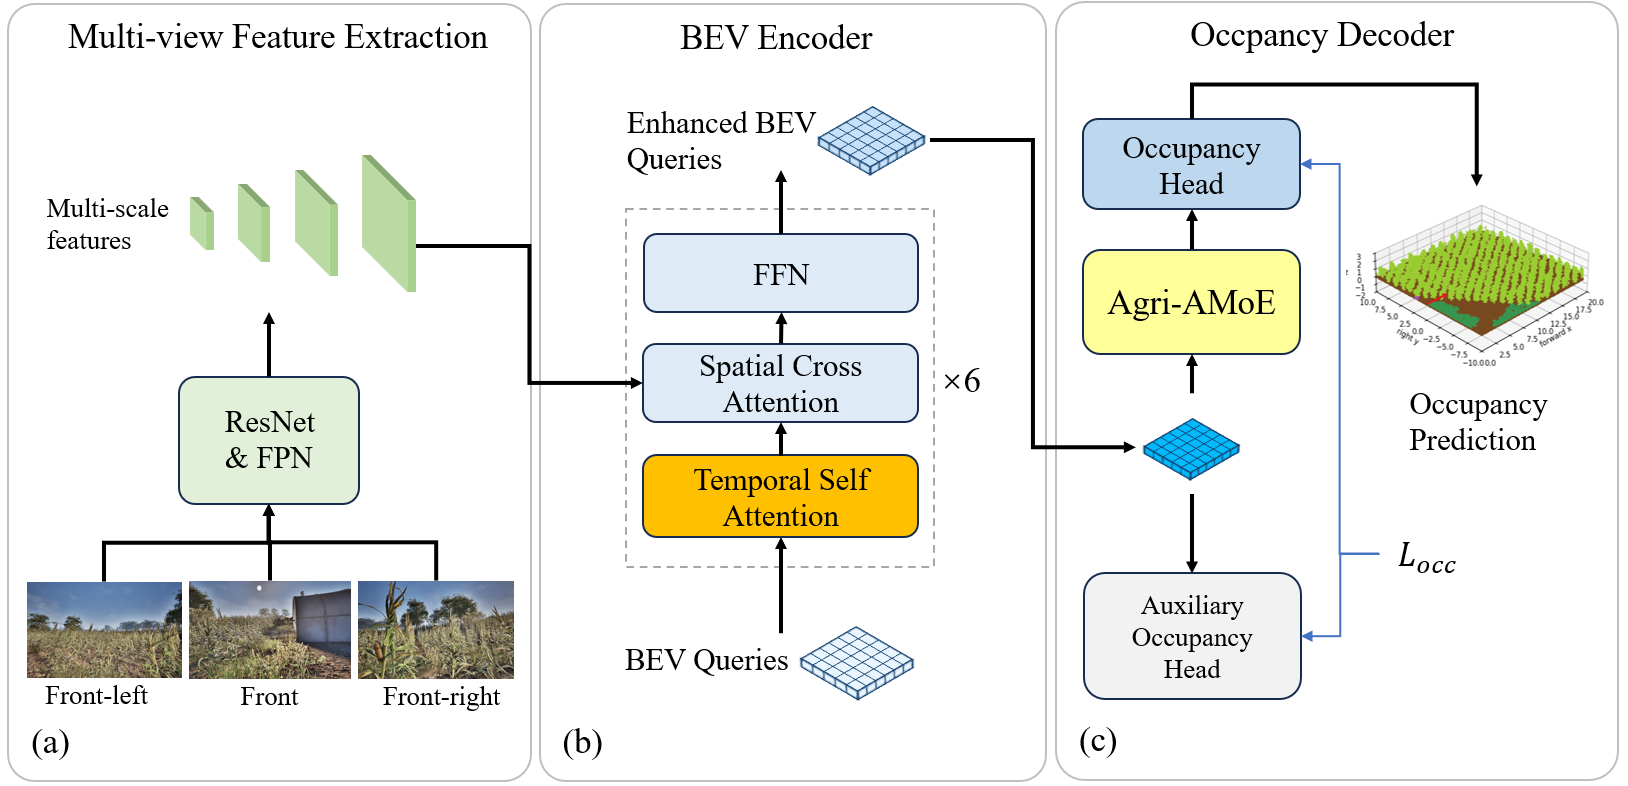
\includegraphics[width=\linewidth]{overview.png}
\caption{Overview of AgriOcc. The six-layer BEV encoder consists of TSA, spatial cross-attention to image features, and feed-forward updates. The final Agri-AMoE branch predicts occupancy, while auxiliary branches provide training supervision.}
\label{fig:overview}
\end{figure}

Our main contributions are as follows:
\begin{enumerate}[leftmargin=1.8em]
\item We develop an Unreal Engine 5-based pipeline for constructing simulated agricultural scenes and collecting 3D semantic occupancy data. The resulting dataset provides six-class voxel annotations of the forward environment in the mobile platform coordinate frame.
\item We propose AgriOcc, which, to our knowledge, is the first 3D semantic occupancy prediction model for the forward field of view of agricultural mobile platforms during field operations. Through end-to-end learning, it maps three forward-facing RGB images to dense semantic voxels in the space ahead, providing a unified 3D representation of agricultural environments.
\item We propose Agri-AMoE, a decoder tailored to agricultural structures, which uses 3D gradient energy and spatial saliency to guide anisotropic expert fusion and enhance structured decoding from a unified BEV representation to semantic occupancy. A crop-aware sampling strategy aligned with the prediction region further improves crop perception and substantially increases crop IoU while keeping the training length fixed.

\end{enumerate}
\section{Related Work}\label{sec:related}
\paragraph{Multi-camera BEV perception}
Bird's-eye-view (BEV) representations map visual evidence from multi-camera images onto a top-down plane in the mobile platform or vehicle coordinate frame, enabling observations from different viewpoints to be fused and used for reasoning and planning in a shared spatial grid.
Vision-based perception methods that use BEV as an intermediate representation align multi-camera image features with this common coordinate frame through predefined spatial queries.
Explicit lifting projects image features into BEV along depth distributions, as in Lift--Splat--Shoot, BEVDet, BEVDepth, and BEVStereo~\citep{philion2020lift,huang2021bevdet,li2022bevdepth,li2022bevstereo}; MatrixVT further investigates efficient multi-camera-to-BEV transformation~\citep{zhou2022matrixvt}.
Query-based methods directly read camera features using 3D reference points, positional embeddings, or cross-view transformations~\citep{wang2022detr3d,li2022petr,liu2023petrv2,li2023fbbev}, and can fuse multimodal information in a shared BEV~\citep{liu2023bevfusion}.
BEVFormer further establishes geometric relationships among BEV queries through spatial cross-attention and temporal self-attention~\citep{li2022bevformer}. These methods provide a foundation for visual perception in a unified coordinate frame.

\paragraph{3D occupancy prediction and efficient representations}
Vision-based 3D occupancy encodes free space and semantic entities as dense or compressed voxel fields. MonoScene, TPVFormer, and VoxFormer perform scene completion through monocular feature lifting, tri-plane representations, and visible sparse voxels, respectively~\citep{cao2022monoscene,huang2023tpvformer,li2023voxformer}; SurroundOcc and OpenOccupancy advance multi-camera dense occupancy prediction and surround-view benchmarks~\citep{wei2023surroundocc,wang2023openoccupancy}.
Because the computational cost of 3D voxels grows rapidly with spatial resolution, subsequent work reduces costs through local--global structures, compact or coarse-to-fine queries, sparse interactions, efficient decoding, and rendering supervision~\citep{zhang2023occformer,ma2024cotr,wang2024panoocc,liu2024sparseocc,tang2024sparseocc,yu2023flashocc,pan2024renderocc}.
Occupancy representations have also been extended to temporal world models: BEVDet4D, OccWorld, IR-WM, and ForecastOcc use cross-frame BEV representations, discrete scene tokens, or historical image observations to predict dynamic environments and future states~\citep{huang2022bevdet4d,zheng2024occworld,mei2025irwm,mohan2026forecastocc}.
These studies demonstrate the value of occupancy as a unified spatial interface, but generally target omnidirectional traffic environments and rely on wider camera coverage or historical motion information.

\paragraph{Agricultural and off-road 3D datasets}
Common urban 3D perception datasets include KITTI~\citep{geiger2012kitti}, SemanticKITTI~\citep{behley2019semantickitti}, and nuScenes~\citep{caesar2020nuscenes}, but their sensor layouts, class compositions, and road structures differ from those of farmland.
Public agricultural datasets mostly target crop-row detection, 2D semantic segmentation, instance segmentation, or specific operational objectives, and rarely provide both multi-camera calibration and dense 3D semantic voxels. The off-road dataset RELLIS-3D~\citep{jiang2020rellis} also primarily serves multimodal segmentation and mapping.
The CARLA virtual-driving platform~\citep{dosovitskiy2017carla}, domain randomization~\citep{tobin2017domainrandomization,peng2018sim2real}, and semantically consistent domain adaptation~\citep{hoffman2018cycada} show that simulation environments can substantially alleviate the high costs and long cycles of real-world data collection, which are particularly challenging in agriculture.
ORAD-3D provides a real-world 3D occupancy benchmark covering farmland, woodland, grassland, and roads~\citep{chen2025orad3d}, enabling validation in real scenes in this work.
Existing agricultural and off-road 3D perception studies mostly use LiDAR or monocular cameras, with sensor configurations and task definitions that differ from our dense semantic occupancy prediction using multiple forward-facing cameras. They are therefore not included in our experimental comparison protocol. To our knowledge, methods that directly predict dense 3D semantic occupancy in the mobile platform coordinate frame from multiple forward-facing cameras for the forward field of view of agricultural mobile platforms during field operations remain unavailable.

\section{Method}\label{sec:method}

\subsection{Task definition}\label{sec:task}
We focus on the most common forward field of view of agricultural mobile platforms during field operations: images from forward, forward-left, and forward-right cameras are used to predict 3D semantic occupancy over the $15\,$m region ahead.
Given three synchronized images at time $t$, $\I_t=\{I_t^{\mathrm{FL}},I_t^{\mathrm{F}},I_t^{\mathrm{FR}}\}$, camera intrinsics and extrinsics, and the mobile platform coordinate frame, the objective is to predict semantic occupancy in the forward region

\begin{equation}
\B=[0,15]\times[-7.5,7.5]\times[-2,3]~\mathrm{m}
\end{equation} 
The voxel resolution is $0.2~\mathrm{m}$, yielding an output grid of $75\times75\times25$. Each valid voxel $v\in\V$ has a label $y_v\in\{0,\ldots,5\}$ denoting one of six classes: free space, crop, soil-covered ground, drivable area, other vegetation, and other obstacles.

\subsection{Simulation data-acquisition system and AgriOcc-Dataset}\label{sec:dataset_construction}
\subsubsection{Farmland simulation data-acquisition system}\label{sec:synthetic}
To alleviate the difficulty of agricultural mobile platform data collection arising from diverse crop types and long acquisition periods, we first construct a parameterized farm simulation environment in Unreal Engine 5, as illustrated in Fig.~\ref{fig:synthetic}.
The scenes contain common elements including farmland, roads, terrain, crops, houses, and fences. Crop instances are arranged on a grid according to planting boundaries, row spacing, and plant spacing.
For each scene, the system first selects assets corresponding to the crop category and growth stage. It then randomizes plant scale, orientation, row and plant spacing, positional perturbations, and missing-plant ratios while preserving plausible field structures and agronomic constraints, simulating diverse growth conditions, densities, and field distributions.

Three synchronized RGB sensors are then mounted on an autonomous tractor, looking forward-left, forward, and forward-right to provide multi-view observations along the direction of travel.
Their mounting height, field of view, resolution, and sampling frequency can be configured jointly. Camera intrinsics and extrinsics, vehicle poses, speeds, and the current scene configuration are recorded synchronously during acquisition, ensuring temporal and spatial consistency among images, vehicle states, and occupancy ground truth.

\begin{figure}[pos=htbp]
\centering
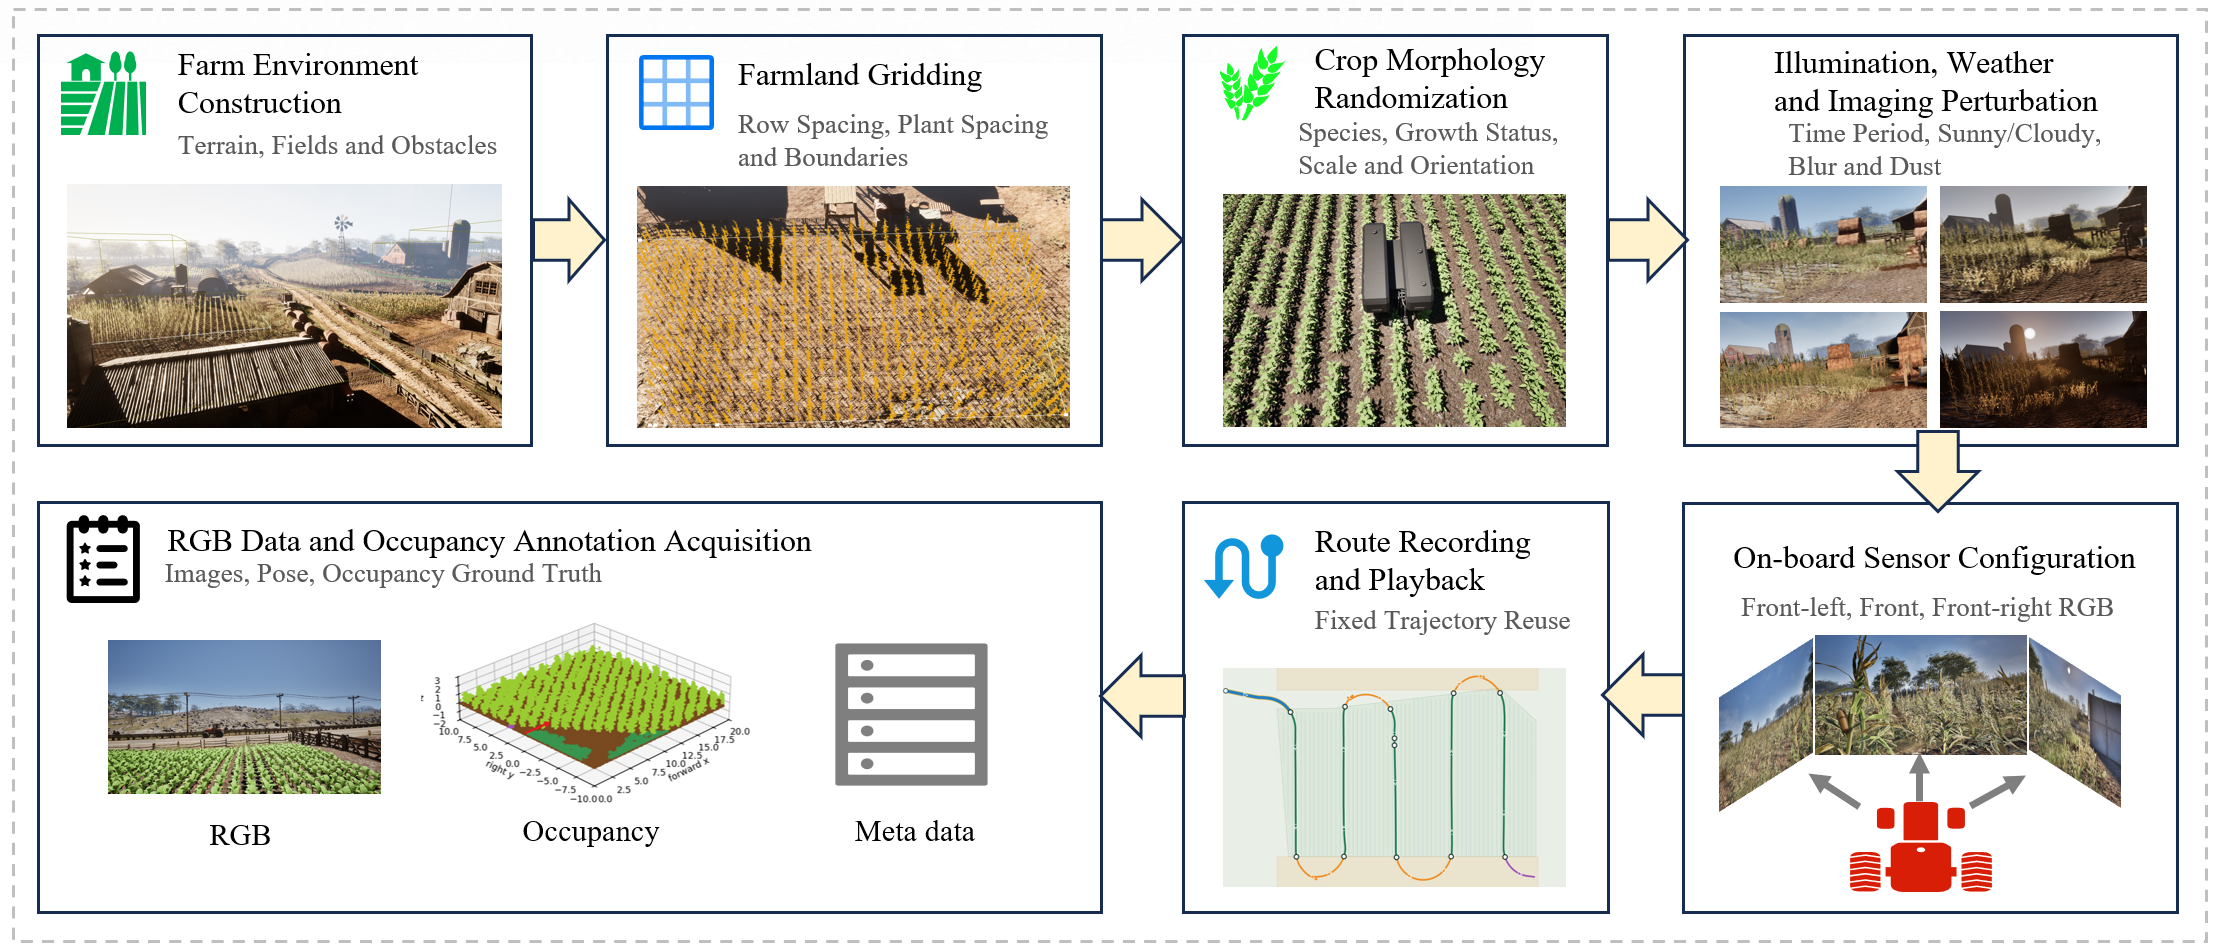
\includegraphics[width=1\linewidth]{synthetic.png}
\caption{Construction pipeline of the farmland simulation data-acquisition system.}
\label{fig:synthetic}
\end{figure}

During data acquisition, we first record several tractor trajectories through the fields and then replay each route under different combinations of crop type, growth stage, time of day, and weather, generating diverse combinations of field scenes and motion trajectories.
To reduce appearance discrepancies between simulation and real acquisition, the system additionally applies imaging perturbations to RGB images with prescribed probabilities, including motion blur, lens stains, and airborne dust particles.
Unlike real-world datasets such as nuScenes, the simulation engine directly exports camera poses, scene semantics, and voxel occupancy states, avoiding complex procedures such as manual per-frame point-cloud semantic annotation, multi-frame spatiotemporal point-cloud registration, and voxel-label generation.
For each frame, the system divides the forward space in the vehicle-local coordinate frame into a regular 3D voxel grid and automatically generates dense occupancy ground truth from scene geometry and semantic labels.
Raw environmental semantics are merged into six task-specific classes: free space, crop, soil-covered ground, drivable area, other vegetation, and other obstacles.
Each sample thus contains RGB images from three views, corresponding 3D semantic occupancy labels, and pose and scene-parameter metadata, forming a multimodal farmland dataset for training and evaluating visual occupancy prediction.

\subsubsection{AgriOcc-Dataset}\label{sec:agriocc_dataset}
Following this process, we construct AgriOcc-Dataset, a multi-view 3D semantic occupancy dataset for agricultural mobile platforms operating in fields.
Each sequence contains synchronized forward, forward-left, and forward-right RGB images, camera intrinsics and extrinsics, mobile platform poses, semantic occupancy labels, and valid-voxel masks.
At loading time, labels are mapped to the six classes free, crop, soil\_ground, drivable, other\_vegetation, and other\_obstacle, and forward voxel supervision is generated in the mobile platform coordinate frame.

 
The dataset contains 298 simulated driving sequences recorded at 10 Hz, totaling approximately 194k frames.
To avoid excessive repetition of similar scenes, we downsample to 2 Hz, obtaining 38.8k samples. Among them, 248 sequences (32,385 frames) are used for training and 50 sequences (6,477 frames) for validation.
The data cover ten crops: cabbage, carrot, corn, cucumber, potato, radish, red beet, sunflower, tomato, and wheat. Each crop includes early, mid, and mature growth stages; dawn, morning, noon, evening, and night; and cloudy and sunny weather. Figure~\ref{fig:crop_distribution} shows the crop composition of the full dataset.

\begin{figure}[pos=htbp]
\centering
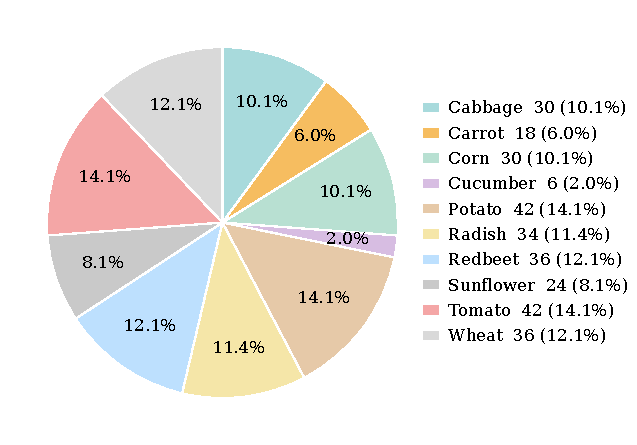
\includegraphics[width=0.5\linewidth]{crop_distribution.pdf}
\caption{Crop composition of AgriOcc-Dataset. Sector area indicates the proportion of each crop.}
\label{fig:crop_distribution}
\end{figure}

\begin{figure}[pos=htbp]
\centering
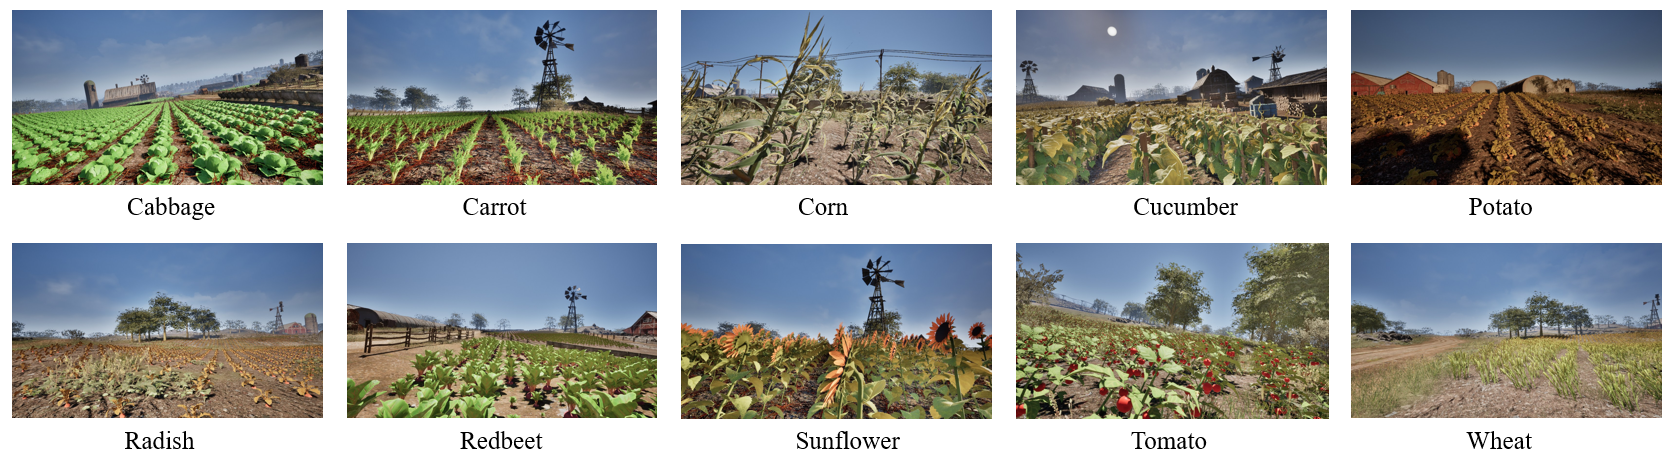
\includegraphics[width=\linewidth]{dataset.png}
\caption{Scene examples of the ten crops in AgriOcc-Dataset.}
\label{fig:dataset}
\end{figure} 

\subsection{Overview of AgriOcc}\label{sec:architecture}
Figure~\ref{fig:overview} illustrates the overall pipeline.
The input tensor has shape $B\times3\times3\times288\times512$, where $B$ is the batch size. Each sample contains three cameras looking forward, forward-left, and forward-right, with three color channels and an image resolution of $512\times288$.
During image encoding, the batch and camera dimensions are merged, and ResNet-101--FPN outputs four feature levels with 256 channels each.
A six-layer BEV encoder then aggregates these image features using $75\times75$ queries. After successive self-attention and spatial cross-attention updates, it outputs $75\times75$ BEV tokens with 256 channels.
Agri-AMoE lifts these BEV tokens into a 3D feature volume and predicts six-class logits at 25 height bins. The final output has shape $B\times75\times75\times25\times6$, and a class-wise argmax yields the semantic grid.
Crop-aware sampling increases exposure to crop voxels during training.

\subsection{BEV encoding}\label{sec:bev}
Occlusion, field-of-view boundaries, and missing local observations affect projection from the three agricultural camera views. Independently mapping each spatial position to the occupancy head can therefore compromise spatial consistency.
Following BEVFormer's basic architecture~\citep{li2022bevformer}, we alternately update queries through adaptive BEV sampling and cross-view projection.
Temporal Self-Attention (TSA) enables information exchange among BEV queries, while Spatial Cross-Attention (SCA) uses BEV queries to index and aggregate visual information at corresponding locations in multi-camera image features.
Each layer performs

\begin{equation}
\begin{aligned}
\widetilde{\bm Q}^{l}&=\operatorname{LN}\!\left(\operatorname{TSA}(\bm Q^{l-1})\right),\\
\widehat{\bm Q}^{l}&=\operatorname{LN}\!\left(\operatorname{SCA}(\widetilde{\bm Q}^{l},\{\bm F_s\},\Pi)\right),\\
\bm Q^l&=\operatorname{LN}\!\left(\widehat{\bm Q}^{l}+\operatorname{FFN}(\widehat{\bm Q}^{l})\right),
\end{aligned}
\end{equation}
where $l=1,\ldots,6$, $\bm F_s$ denotes image features at level $s$, $\Pi$ denotes the camera projection relationships, and LN denotes layer normalization. Both TSA and SCA include internal residual connections.

We use only current-frame images. In the absence of a historical BEV, both internal value slots of TSA are filled with the current BEV queries, from which 2D sampling offsets and attention weights are predicted.
Although the two slots share the same information source, learnable offsets still allow each query to sample and aggregate features from different BEV positions with adaptive weights. The module thus retains adaptive spatial interaction in the single-frame setting.
The first TSA layer operates on learnable BEV queries. Subsequent layers further aggregate BEV features that have already incorporated image evidence in the preceding layer, allowing observations at different positions to propagate progressively as encoder layers are stacked.

Retaining TSA is particularly important in agricultural scenes: occlusion, field-of-view boundaries, and projection errors in the three forward-facing images cause uneven observation quality across BEV positions, while crop rows, furrows, and ground regions exhibit strong spatial correlations.
TSA allows queries to adaptively select contextual positions based on their features, enabling weakly observed regions to use information from surrounding positions and helping preserve the continuity of crop rows and ground layouts. Residual connections preserve the original representation at each position.
Complementing TSA, SCA projects pillar reference points into the three images and samples and aggregates visual evidence across valid views and multiple feature scales.
Alternating these updates enables both multi-view image-evidence aggregation and structural interaction within BEV, providing spatially consistent representations for subsequent 3D occupancy decoding. This motivates retaining TSA even in our single-frame setting.

\subsection{Agricultural Structure-Adaptive Mixture-of-Experts decoder}\label{sec:amoe}
Farmland occupancy exhibits pronounced anisotropy: crop rows and furrows show long-range continuity and periodic alternation on the ground plane, while crop canopies, soil, and obstacles have different boundary shapes along the height dimension.
In particular, inter-plant gaps and crop--free-space boundaries often occupy only a small number of voxels. If 2D BEV tokens are independently mapped directly to classes at each height, the decoder struggles to coordinate planar details and vertical structures across neighboring positions, resulting in oversmoothing in fine-grained regions.
The final occupancy head must therefore both recover the height dimension and adaptively select appropriate receptive fields and directional modeling according to the complexity of local 3D structures.

Inspired by the use of mixtures of experts for occupancy decoding in \citet{shi2026oneocc}, we design the Agricultural Structure-Adaptive Mixture-of-Experts 3D occupancy decoder (Agri-AMoE).
Rather than defining experts for general urban scenes, we tailor their forms to the anisotropic planar, vertical, and contextual structures of farmland. Interpretable gradient energy serves as a routing signal, directly linking expert specialization to agricultural structures such as crop rows, furrows, and canopies.
The final-layer BEV features $\bm{Q}\in\R^{B\times HW\times C}$ are first linearly mapped and reshaped into a 3D feature volume with $C_a$ channels:

\begin{equation}
\bm{F}_0=\operatorname{reshape}(W_{\mathrm{lift}}\bm{Q})\in\R^{B\times C_a\times Z\times H\times W}.
\end{equation}
Here, $C$ is the channel dimension of the input BEV tokens, $H$ and $W$ are the two planar dimensions of the BEV grid, and $Z$ is the number of height bins. $W_{\mathrm{lift}}$ is a learnable lifting map, and $\operatorname{reshape}(\cdot)$ only rearranges the mapped tokens into a 3D volume.
We use $C_a=96$ and $Z=25$. Global 3D pooling is first applied to $\bm{F}_0$, and an MLP generates channel-attention weights to enhance the 3D volume features:

\begin{equation}
\bm{F}=\bm{F}_0\odot\sigma\!\left(f_c(\operatorname{GAP}(\bm{F}_0))\right).
\end{equation}
where $\operatorname{GAP}$ denotes global average pooling over the $Z$, $H$, and $W$ dimensions, $f_c$ is a learnable channel mapping, $\sigma$ is the sigmoid function, and $\odot$ denotes element-wise multiplication.
The enhanced features $\bm{F}$ are fed simultaneously to three parallel anisotropic experts and the routing branch.
All three experts take $\bm{F}$ as input: $\mathcal{E}_1$ uses a $1\times3\times3$ depthwise separable convolution to encode planar details between plants, $\mathcal{E}_2$ uses a $3\times1\times1$ convolution to encode vertical structures, and $\mathcal{E}_3$ uses a $1\times3\times3$ convolution with dilation 2 to encode broader planar context.

The router then assigns expert weights to each voxel based on the spatial saliency and local structural variation of $\bm{F}$.
Spatial saliency is computed from the channel-wise mean and maximum of $\bm{F}$ through a $3\times3\times3$ convolutional spatial mapping $f_s$:

\begin{equation}
\bm{S}=\sigma\!\left(f_s([\operatorname{mean}_c(\bm{F}),\operatorname{max}_c(\bm{F})])\right).
\end{equation}
where $\operatorname{mean}_c$ and $\operatorname{max}_c$ denote mean and maximum aggregation along the channel dimension, respectively, and $\bm{S}$ is a voxel-wise spatial saliency map.
To further align expert selection with 3D structural complexity, the router also computes the finite-difference energy of $\bm{F}$ along the three spatial directions:

\begin{equation}
\bm{E}=\operatorname{mean}_c\!\left((\nabla_x\bm{F})^2+(\nabla_y\bm{F})^2+(\nabla_z\bm{F})^2\right).
\end{equation}
where $\nabla_x$, $\nabla_y$, and $\nabla_z$ denote gradients along the three spatial directions, so $\bm{E}$ measures voxel-wise local structural variation.
Taking $[\log(1+\bm{E}),\bm{S}]$ as input, the router outputs three normalized expert weights at temperature $\tau=1$:

\begin{equation}
\bm{\alpha}=\operatorname{Softmax}\!\left(g([\log(1+\bm{E}),\bm{S}]) / \tau\right),
\end{equation}
where $g$ is a three-output routing mapping consisting of two $1\times1\times1$ convolutions, group normalization, and ReLU, and $\alpha_k$ is the weight of expert $k$ at each voxel.
Finally, these routing weights combine the outputs of all three experts, which have already been computed:

\begin{equation}
\bm{F}'=\operatorname{ReLU}\!\left(\bm{F}+\operatorname{GN}\!\left(\sum_{k=1}^{3}\alpha_k\mathcal{E}_k(\bm{F})\right)\right),\qquad
\bm{O}=W_o\bm{F}',
\end{equation}
where $\operatorname{GN}$ denotes group normalization, $\operatorname{ReLU}$ is the nonlinear activation, and $W_o$ is a $1\times1\times1$ classification convolution.
The final semantic logits are $\bm{O}\in\R^{B\times6\times Z\times H\times W}$. Figure~\ref{fig:agri-amoe} illustrates the module architecture.

\begin{figure}[pos=htbp]
\centering
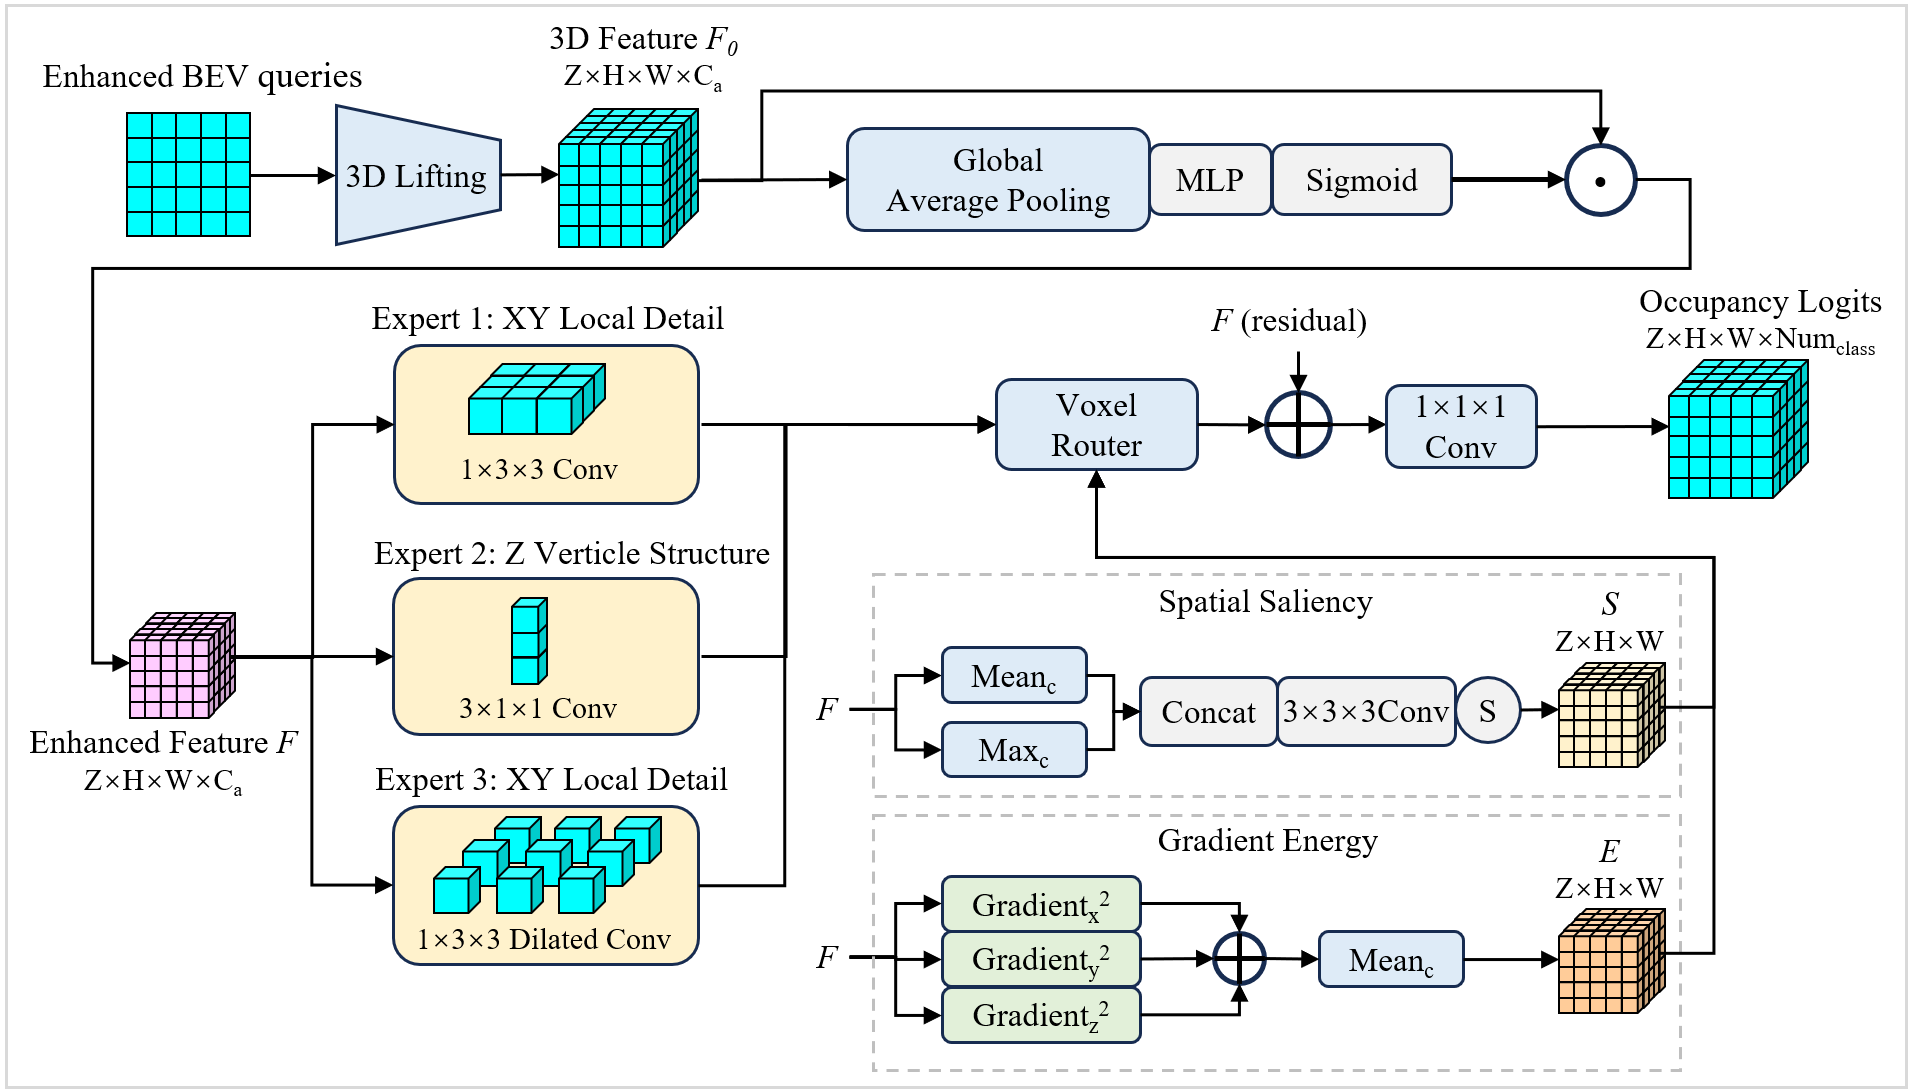
\includegraphics[width=\linewidth]{agri-amoe.png}
\caption{Agri-AMoE 3D occupancy decoder. The 2D BEV tokens are lifted into a 3D volume and first enhanced by channel attention. The enhanced features are fed in parallel to three anisotropic experts and are also used to generate spatial saliency and gradient energy along three directions for voxel-wise routing weights. The three expert outputs are combined by weighted summation and residual fusion before final classification.}
\label{fig:agri-amoe}
\end{figure}

\subsection{Crop-aware sampling aligned with the prediction region}\label{sec:cropsample}
Accurate crop perception is crucial for agricultural mobile platforms traveling along crop rows. In farmland samples, common voxel classes such as soil and roads are abundant, whereas the number of crop voxels varies substantially across scenes.
Samples with a low proportion of crop voxels provide extensive ground and free-space supervision but insufficient observations of plant boundaries, reducing crop perception accuracy.
We therefore propose a training-time data-sampling strategy that replaces a small quota of samples to increase exposure to crop supervision.
For training frame $i$, we first count valid crop voxels within the prediction region:

\begin{equation}
n_i=\sum_{v\in\V_i}\mathbf 1[y_v=\mathrm{crop}],\qquad
\mathcal D_+=\{i:n_i\ge T\}.
\end{equation}
Here, $T$ is the threshold for selecting samples containing crops. Crop counts from the original larger region cannot be used directly to select training samples for a smaller prediction region.
At each epoch, all $N$ training indices are first randomly permuted. Then, $K=\operatorname{round}(\rho N)$ positions are selected and replaced with indices drawn uniformly with replacement from $\mathcal D_+$.
Positions with $n_i<T$ are prioritized for replacement; if insufficient, the set of candidate positions is expanded.
The epoch length therefore remains identical to that of the baseline sampler, without appending additional training frames.
Our model uses $\rho=0.10$ and $T=500$.

\subsection{Optimization objective}\label{sec:loss}
The three current-frame occupancy output branches are supervised by the same semantic ground truth.
Following common voxel supervision in SurroundOcc and OpenOccupancy~\citep{wei2023surroundocc,wang2023openoccupancy}, each branch uses classification cross-entropy, semantic scaling, geometric scaling, and Lov\'{a}sz-Softmax terms:

\begin{equation}
\mathcal L=\sum_{j=1}^{3}\left(\lambda_{\mathrm{ce}}\mathcal L_{\mathrm{ce}}^{(j)}+
\lambda_{\mathrm{sem}}\mathcal L_{\mathrm{sem}}^{(j)}+
\lambda_{\mathrm{geo}}\mathcal L_{\mathrm{geo}}^{(j)}+
\lambda_{\mathrm{lov}}\mathcal L_{\mathrm{lov}}^{(j)}\right).
\end{equation}
Here, $j$ indexes the output branches. All four $\lambda$ coefficients are set to 1, and cross-entropy uses a class weight of 1 for Free and 5 for each of the other semantic classes.
All terms are computed only over valid voxels; voxels below the ground surface are treated as invalid and excluded.
\section{Experiments}\label{sec:experiments}
\subsection{Data and evaluation protocol}\label{sec:data}
We conduct occupancy experiments on AgriOcc-Dataset, described in Section~\ref{sec:agriocc_dataset}.
The dataset covers 0 m to 15 m along the $x$ axis (forward), $-7.5$ m to 7.5 m along the $y$ axis, and $-2$ m to 3 m along the $z$ axis.
Occupancy labels are defined using $0.2\times0.2\times0.2\,\mathrm{m}$ voxels and six classes: Free, Crop, Soil, Drivable, Other veg., and Other obs.
For class $c$, $\IoU_c=\mathrm{TP}_c/(\mathrm{TP}_c+\mathrm{FP}_c+\mathrm{FN}_c)$; mIoU is the arithmetic mean of the six class IoUs, including Free.
Models from the final training epoch are used for evaluation.
We also evaluate transfer to real environments on the official ORAD-3D test set and its farmland subset, and assess voxel-resolution transfer using independently collected high-resolution simulation data.

\subsection{Implementation details}\label{sec:implementation}
The image encoder uses ResNet-101--FPN initialized with pretrained weights.
Input images have a resolution of $512\times288$. The BEV grid contains $75\times75$ queries with 256 channels, the encoder has 6 layers, and the Agri-AMoE width is 96.
AdamW uses an initial learning rate of $2\times10^{-4}$ and weight decay of 0.01, with cosine decay and linear warm-up over 500 iterations.
We train for 15 epochs on three RTX 4090 GPUs with a global batch size of 24. The main crop-aware sampling configuration is $\rho=0.10,T=500$.
Of the 32,385 training frames, 20,300 meet this crop threshold, and approximately 3,238 positions are replaced at most per epoch.
The compared methods retain their original architectures and optimization objectives, while sharing the prediction region, three forward-facing inputs, image size, data split, and number of training epochs.

\subsection{Comparison with existing methods}\label{sec:comparison}
Table~\ref{tab:main} compares AgriOcc with several state-of-the-art semantic occupancy methods.
SurroundOcc~\citep{wei2023surroundocc}, SparseOcc~\citep{tang2024sparseocc}, and COTR~\citep{ma2024cotr} predict current-frame semantic occupancy, whereas Drive-OccWorld~\citep{yangDrivingOccupancyWorld2025} and IR-WM~\citep{mei2025irwm} jointly predict current and future occupancy.
We retain their historical inputs, future occupancy prediction, and joint trajectory tasks, and compare only their current-frame outputs.
AgriOcc outperforms all compared methods in IoU for every class.

\begin{table}[pos=htbp]
\centering
\caption{3D semantic occupancy performance on AgriOcc-Dataset. IoUs are reported in \%, and inference time in ms/frame.}
\label{tab:main}
\resizebox{\linewidth}{!}{%
\begin{tabular}{lrrrrrrrrr}
\toprule
Method & Params (M) & Inference time & mIoU & Free & Crop & Soil & Drivable & Other veg. & Other obs.\\
\midrule
SurroundOcc & 198.24 & 83.73 & 61.84 & 93.43 & 30.67 & 80.46 & 73.05 & 49.73 & 43.72 \\
SparseOcc & 58.14 & 28.88 & 33.35 & 89.24 & 6.95 & 45.14 & 36.88 & 9.96 & 11.95 \\
COTR & 37.16 & 32.33 & 56.24 & 89.86 & 26.65 & 76.56 & 61.47 & 46.91 & 35.98 \\
Drive-OccWorld & 60.68 & 170.12 & 35.15 & 85.52 & 19.63 & 40.29 & 29.64 & 21.06 & 14.77 \\
IR-WM & 58.42 & 173.83 & 38.62 & 86.93 & 21.20 & 46.68 & 33.01 & 24.68 & 19.25 \\
AgriOcc & 53.03 & 63.34 & 64.08 & 93.55 & 39.38 & 80.57 & 74.38 & 50.69 & 45.91 \\
\bottomrule
\end{tabular}}
\end{table}
 
AgriOcc achieves 64.08\% mIoU, exceeding SurroundOcc's 61.84\% by 2.24 percentage points, a relative improvement of 3.6\%.
Crop IoU increases from 30.67\% to 39.38\%, a gain of 8.71 percentage points; Soil and Drivable IoUs reach 80.57\% and 74.38\%, respectively.
In contrast, IR-WM and Drive-OccWorld are also influenced by their joint future-prediction and planning objectives and therefore offer no advantage in 3D semantic occupancy performance.
SurroundOcc, SparseOcc, and COTR primarily target urban surround-view driving scenes: uniform spatial queries and urban road priors do not readily accommodate inter-row occlusion, slender crops, and fine near-field boundaries in the forward view of agricultural mobile platforms.
IR-WM and Drive-OccWorld instead emphasize world modeling and planning through historical states, action conditioning, and future rollout prediction. For current-frame occupancy prediction, these additional capabilities do not fully translate into voxel accuracy, and joint multi-step optimization increases the difficulty of representation learning.
Their lower current-frame metrics therefore reflect a mismatch in task objectives and inductive biases, rather than limited capability in future-state prediction or planning.

Inference time is measured on a single RTX 4090 with a batch size of 1, averaging model inference time over 50 frames after a 10-frame warm-up.
AgriOcc requires 63.34 ms/frame; although slower than COTR and SparseOcc, it provides substantial accuracy advantages.
With TensorRT FP16 acceleration, AgriOcc achieves an inference time of 6.82 ms/frame, approximately 146.6 FPS, demonstrating strong real-time performance for deployment.

Figures~\ref{fig:comparison} and~\ref{fig:comparison_sparse} compare predictions on the same three scenes.
All methods use the same ground-truth validity mask and semantic colors, with a fixed viewpoint above and directly behind the mobile platform, looking along its direction of travel.
AgriOcc recovers the main ground layout and vegetation regions, improving environmental understanding compared with the other methods.

\begin{figure}[pos=htbp]
\centering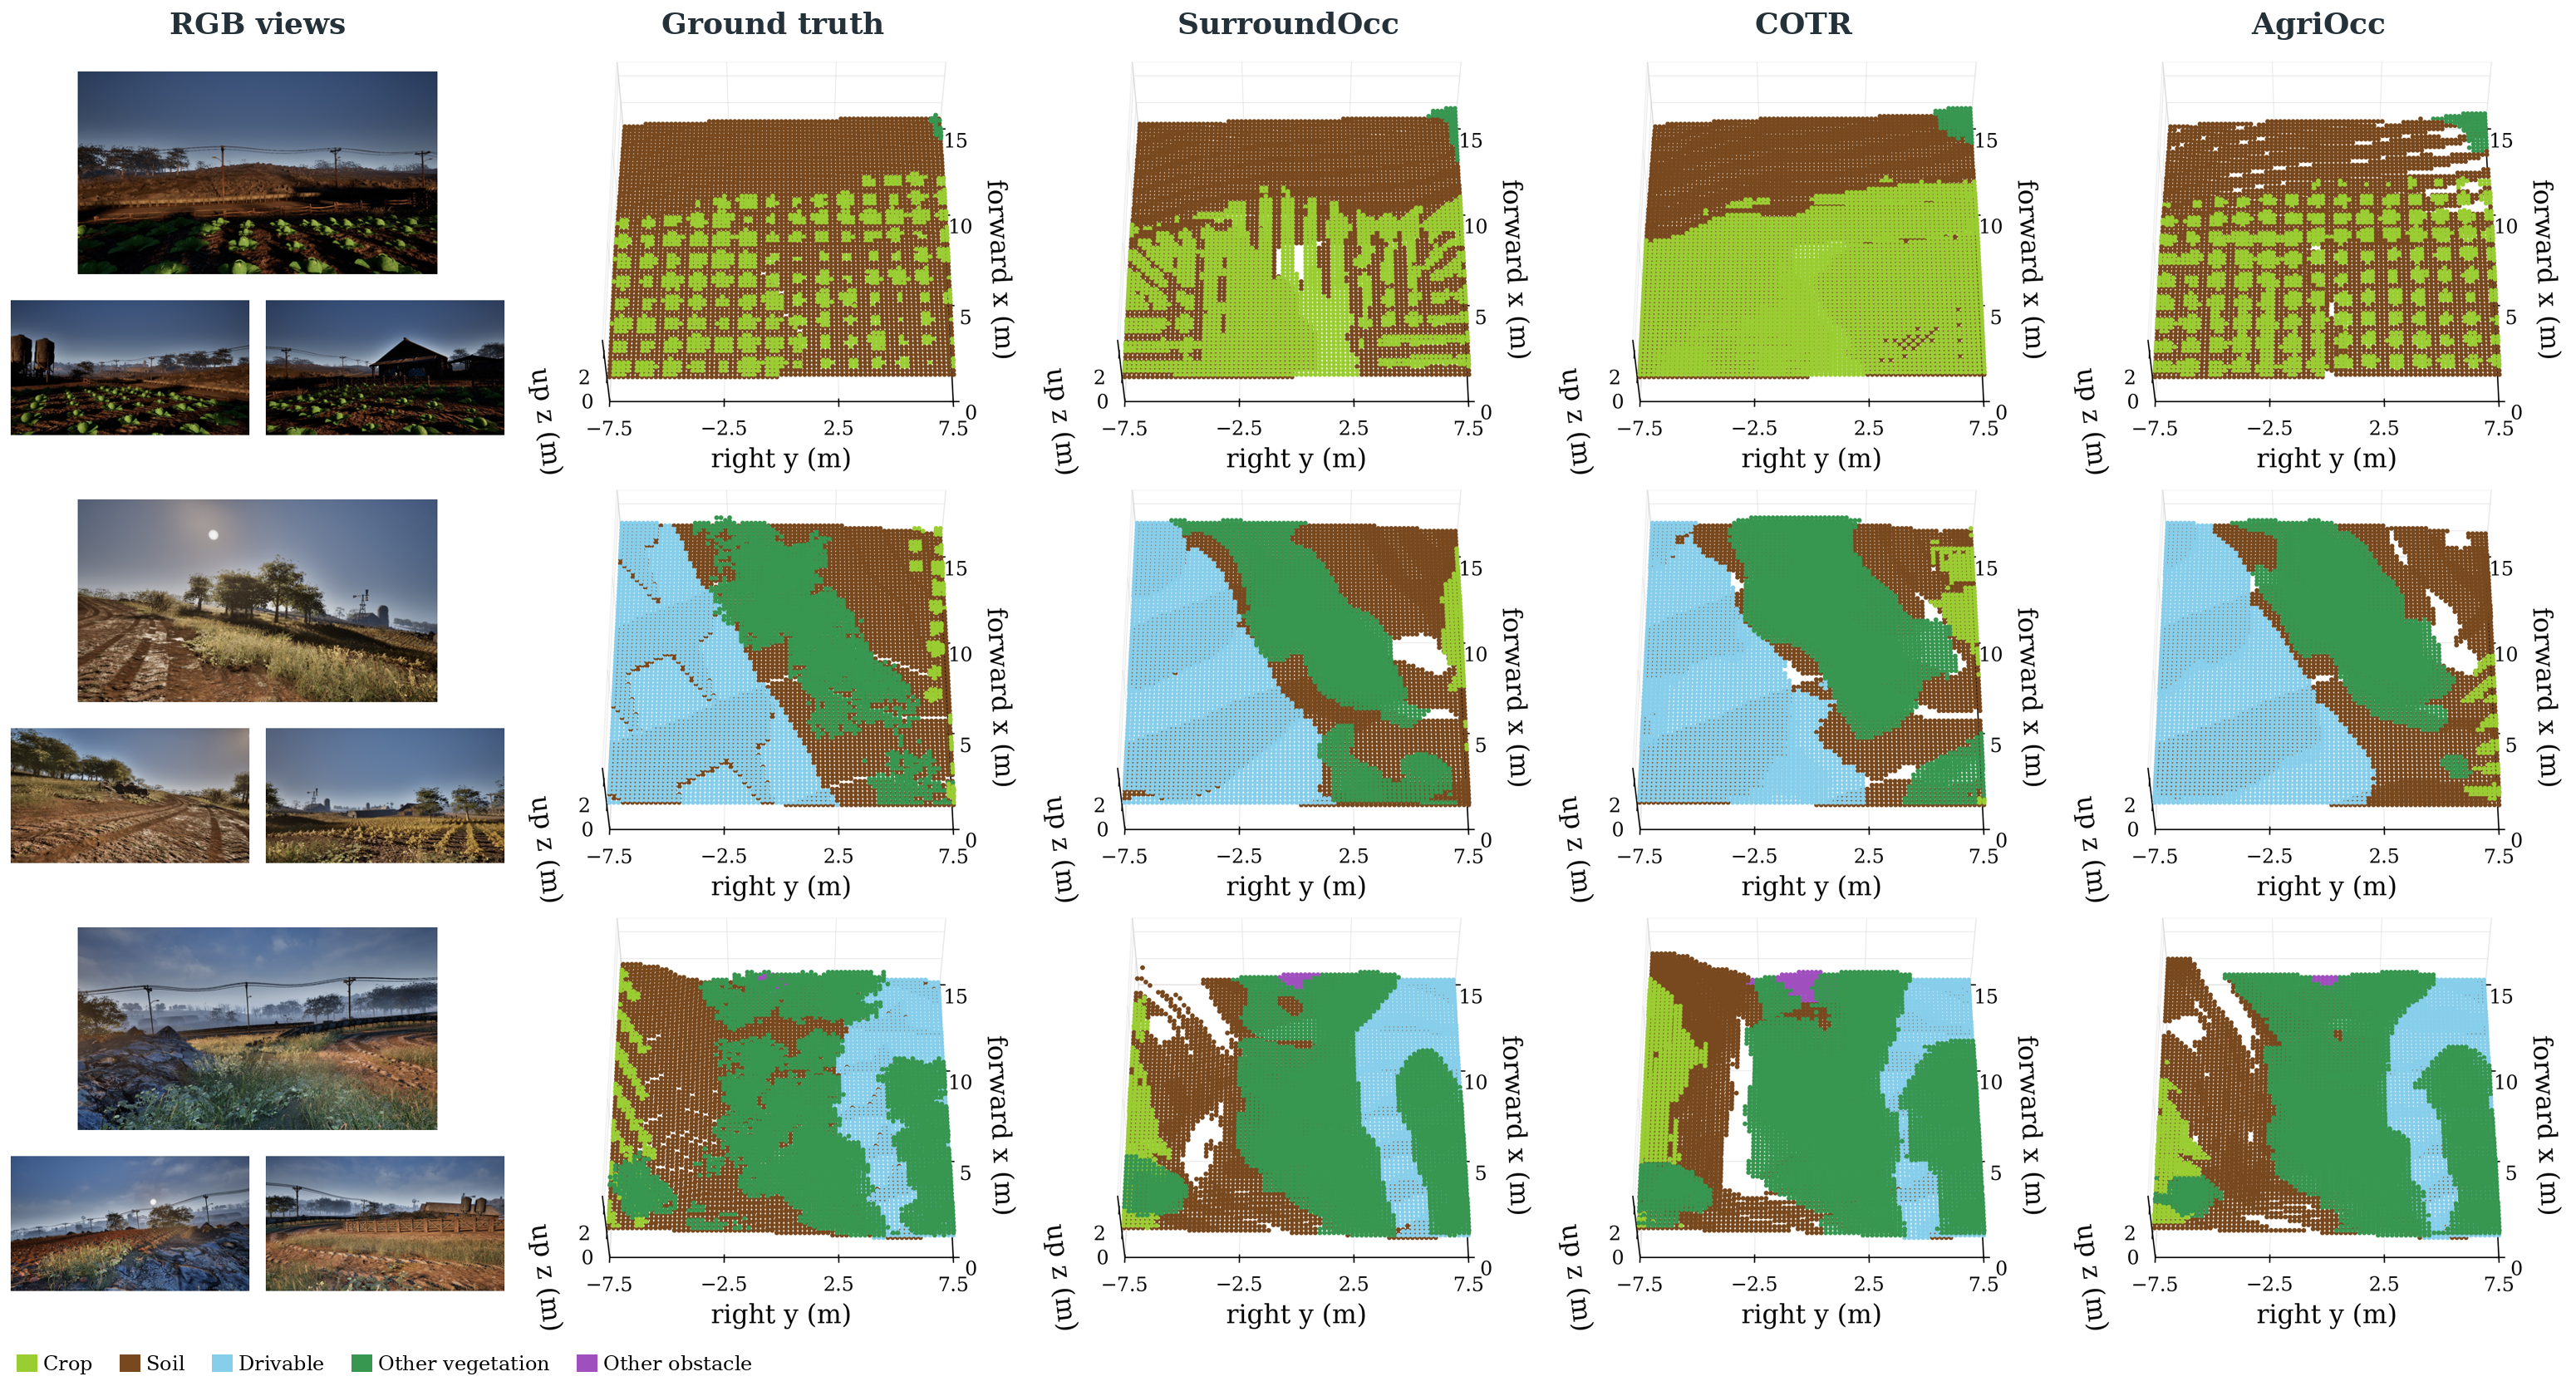
\includegraphics[width=\linewidth]{qualitative_comparison.png}
\caption{Qualitative comparison of current-frame occupancy. From left to right: three-view RGB images, GT, SurroundOcc, COTR, and AgriOcc. All occupancy views share the same viewpoint above and directly behind the mobile platform, spatial extent, and valid-voxel mask.}
\label{fig:comparison}
\end{figure}
\begin{figure}[pos=htbp]
\centering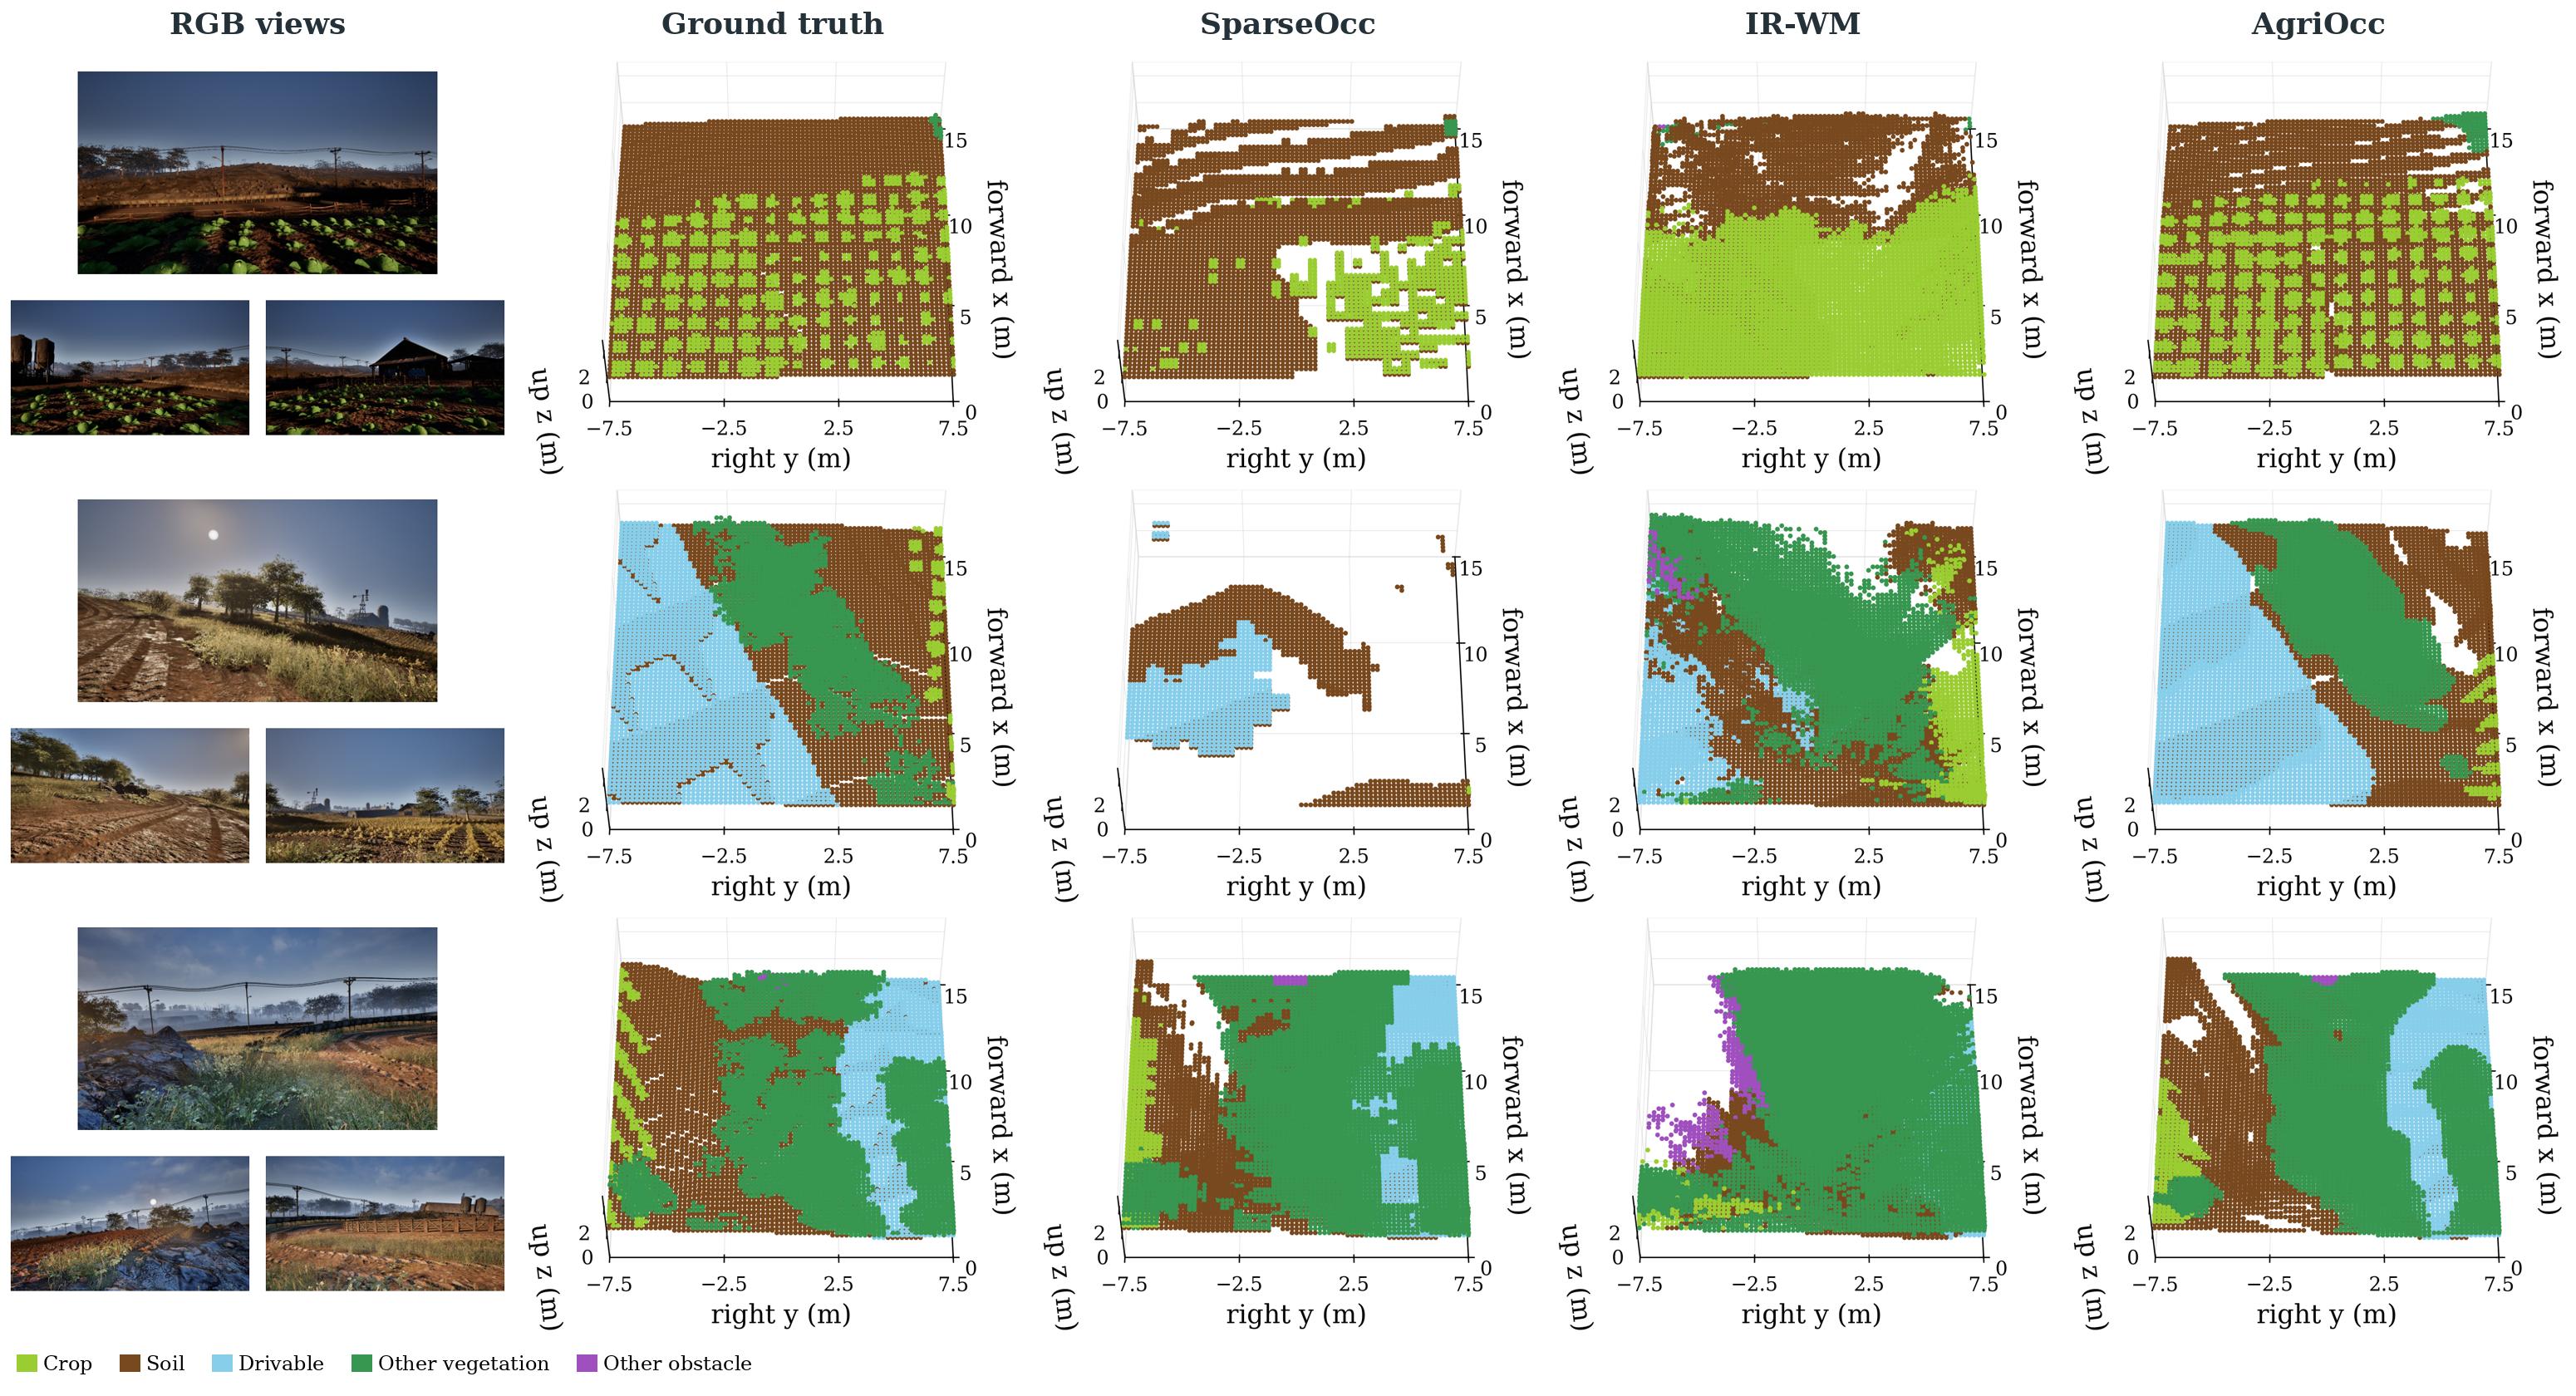
\includegraphics[width=\linewidth]{qualitative_sparse_irwm.png}
\caption{Qualitative comparison with SparseOcc and IR-WM. Columns show RGB images, GT, SparseOcc, IR-WM, and AgriOcc, using the same viewpoint and semantic colors as Fig.~\ref{fig:comparison}.}
\label{fig:comparison_sparse}
\end{figure}

\subsection{Ablations of architecture and training strategy}\label{sec:ablation}

\paragraph{Ablation of main model components}
Table~\ref{tab:ablation} sequentially examines the effects of TSA, Agri-AMoE, and crop-aware sampling.
Base uses the same ResNet-101--FPN, six-layer BEV encoder, and MLP-based occupancy decoder, but removes TSA and the immediately following layer normalization from each encoder layer, retaining only SCA and feed-forward updates.
All configurations share the data split, image inputs, pretrained initialization, number of training epochs, and evaluation protocol.
Adding TSA increases the number of trainable parameters from 50.99 M to 52.37 M, raises mIoU from 60.36\% to 62.76\%, and improves crop IoU from 30.03\% to 35.76\%, indicating that adaptive spatial interaction among current-frame BEV queries benefits occupancy prediction.
Replacing the final occupancy decoder with Agri-AMoE adds only 0.66 M parameters and further increases mIoU to 64.20\% and crop IoU to 38.93\%, gains of 1.44 and 3.17 percentage points, respectively.
Further applying crop-aware sampling increases crop IoU to 39.38\%, while mIoU decreases slightly to 64.08\%, reflecting a trade-off between crop recognition and overall accuracy.

\begin{table}[pos=htbp]
\centering
\caption{Ablation of main model components. Base excludes TSA, Agri-AMoE, and crop-aware sampling. Subsequent rows successively add TSA, Agri-AMoE, and crop-aware sampling to the preceding configuration.}
\label{tab:ablation}
\begin{tabular}{lrrrr}
\toprule
Configuration & Sampling $(\rho,T)$ & Trainable params (M) & mIoU(\%) & Crop IoU(\%)\\
\midrule
Base & -- & 50.99 & 60.36 & 30.03\\
Base + TSA & -- & 52.37 & 62.76 & 35.76\\
Base + TSA + Agri-AMoE & -- & 53.03 & 64.20 & 38.93\\
AgriOcc & $(0.10,500)$ & 53.03 & 64.08 & 39.38\\
\bottomrule
\end{tabular}
\end{table}

\paragraph{Ablation of the sampling strategy}
Our experiments show that increasing exposure to crop samples does not necessarily improve IoU for all classes.
Table~\ref{tab:sampling} reports results under different sampling settings using the Base + TSA + Agri-AMoE architecture.
With $T=500$ fixed, increasing $\rho$ from $0.10$ to $0.20$ raises crop IoU only from 39.38\% to 39.46\%, while mIoU drops to 63.23\%.
A larger quota reduces exposure to some background samples and changes the balance of class decisions. We therefore adopt the more balanced setting of $0.10$.

\begin{table}[pos=htbp]
\centering
\caption{Sampling sensitivity results.}
\label{tab:sampling}
\begin{tabular}{lrrr}
\toprule
Model & $(\rho,T)$ & mIoU(\%) & Crop IoU(\%)\\
\midrule
Base + TSA + Agri-AMoE & No crop-aware sampling & 64.20 & 38.93\\
Base + TSA + Agri-AMoE & $(0.10,500)$ & 64.08 & 39.38\\
Base + TSA + Agri-AMoE & $(0.15,500)$ & 63.67 & 39.02\\
Base + TSA + Agri-AMoE & $(0.20,500)$ & 63.23 & 39.46\\
\bottomrule
\end{tabular}
\end{table}

\subsection{Real-world transfer and qualitative analysis}\label{sec:sim2real}
\subsubsection{Transfer from simulation to a real-world dataset}\label{sec:orad_transfer}
To further validate the real-world effectiveness of models trained on simulation data, we transfer the model trained on AgriOcc-Dataset to ORAD-3D~\citep{chen2025orad3d} and evaluate it on the official test set and its farmland subset.
The ORAD-3D occupancy grid has shape $100\times100\times16$ and nine voxel classes, following its official annotation protocol.
AgriOcc is designed for three forward-facing cameras, which do not match ORAD-3D's surround-view sensor configuration, and the two datasets use different class taxonomies.
We therefore use only the BEV embedding from the center forward-facing camera, replace the occupancy head to match the target grid shape and number of classes, and perform alignment training on the ORAD-3D training set.

We adapt the model pretrained on AgriOcc-Dataset to the target domain and compare it with AgriOcc trained from scratch and the baseline models in the ORAD-3D paper.
Table~\ref{tab:orad} reports results on the official ORAD-3D test set and the farmland subset selected from it.
\texttt{Test} is computed over the full class set, while \texttt{Test\_farm} is computed over classes present in the farmland subset.
For comparability with the semantic mIoU reported in the ORAD-3D paper, we additionally report Test mIoU excluding Free. The OpenOcc, OccFormer, and SurroundOcc results are taken from the ORAD-3D paper~\citep{chen2025orad3d}.
Using the same complete target-domain training set, AgriOcc pretrained on AgriOcc-Dataset requires only 2 adaptation epochs to achieve 11.17\% on \texttt{Test (w/o Free)}, exceeding the 9.01\% obtained by training from scratch and the 7.60\% reported in the ORAD-3D paper, while reducing target-domain training time from 54.1 to 18.5 minutes.
This indicates that image--BEV geometric and 3D semantic priors acquired through pretraining on synthetic agricultural data can transfer effectively to real off-road scenes, improving semantic occupancy prediction at a lower target-domain adaptation cost.

Table~\ref{tab:orad} uses results from an independent test set.
Test averages a fixed set of nine classes, and Test w/o Free averages the eight classes excluding Free.

\begin{table}[pos=htbp]
\centering
\caption{Sim-to-real transfer results on ORAD-3D (\%). Both AgriOcc models use the complete ORAD-3D training set and only the center forward-facing camera. The transfer model is initialized with weights pretrained on AgriOcc-Dataset and adapted for 2 epochs.
\texttt{Test (w/o Free)} denotes mIoU excluding Free, following the ORAD-3D paper; \texttt{Test} denotes mIoU over all nine classes; and \texttt{Test\_farm} denotes mIoU over the classes present in the farmland subset.
The OpenOcc, OccFormer, and SurroundOcc results are taken from the ORAD-3D paper.}

\label{tab:orad}
\fontsize{9}{11}\selectfont
\setlength{\tabcolsep}{2.6pt}
\begin{tabular}{lrrrr}
\toprule 
Method & Training time (min) & Test (w/o Free) & Test & Test\_farm \\
\midrule
OpenOcc~\citep{jiang2024openocc} & -- & 5.83 & -- & -- \\
OccFormer~\citep{zhang2023occformer} & -- & 7.45 & -- & -- \\
SurroundOcc~\citep{wei2023surroundocc} & -- & 7.60 & -- & -- \\
\midrule
AgriOcc (from scratch) & 54.1 & 9.01 & 18.16 & 31.83 \\
\midrule
AgriOcc (pretrained transfer) & 18.5 & \textbf{11.17} & \textbf{20.11} & 39.45 \\
\bottomrule
\end{tabular}
\end{table}

Figure~\ref{fig:orad} shows the same set of real farmland test frames. Both sets of predictions capture the main road layout, but local occupancy boundaries and small or rare classes remain challenging.
\begin{figure}[pos=htbp]
\centering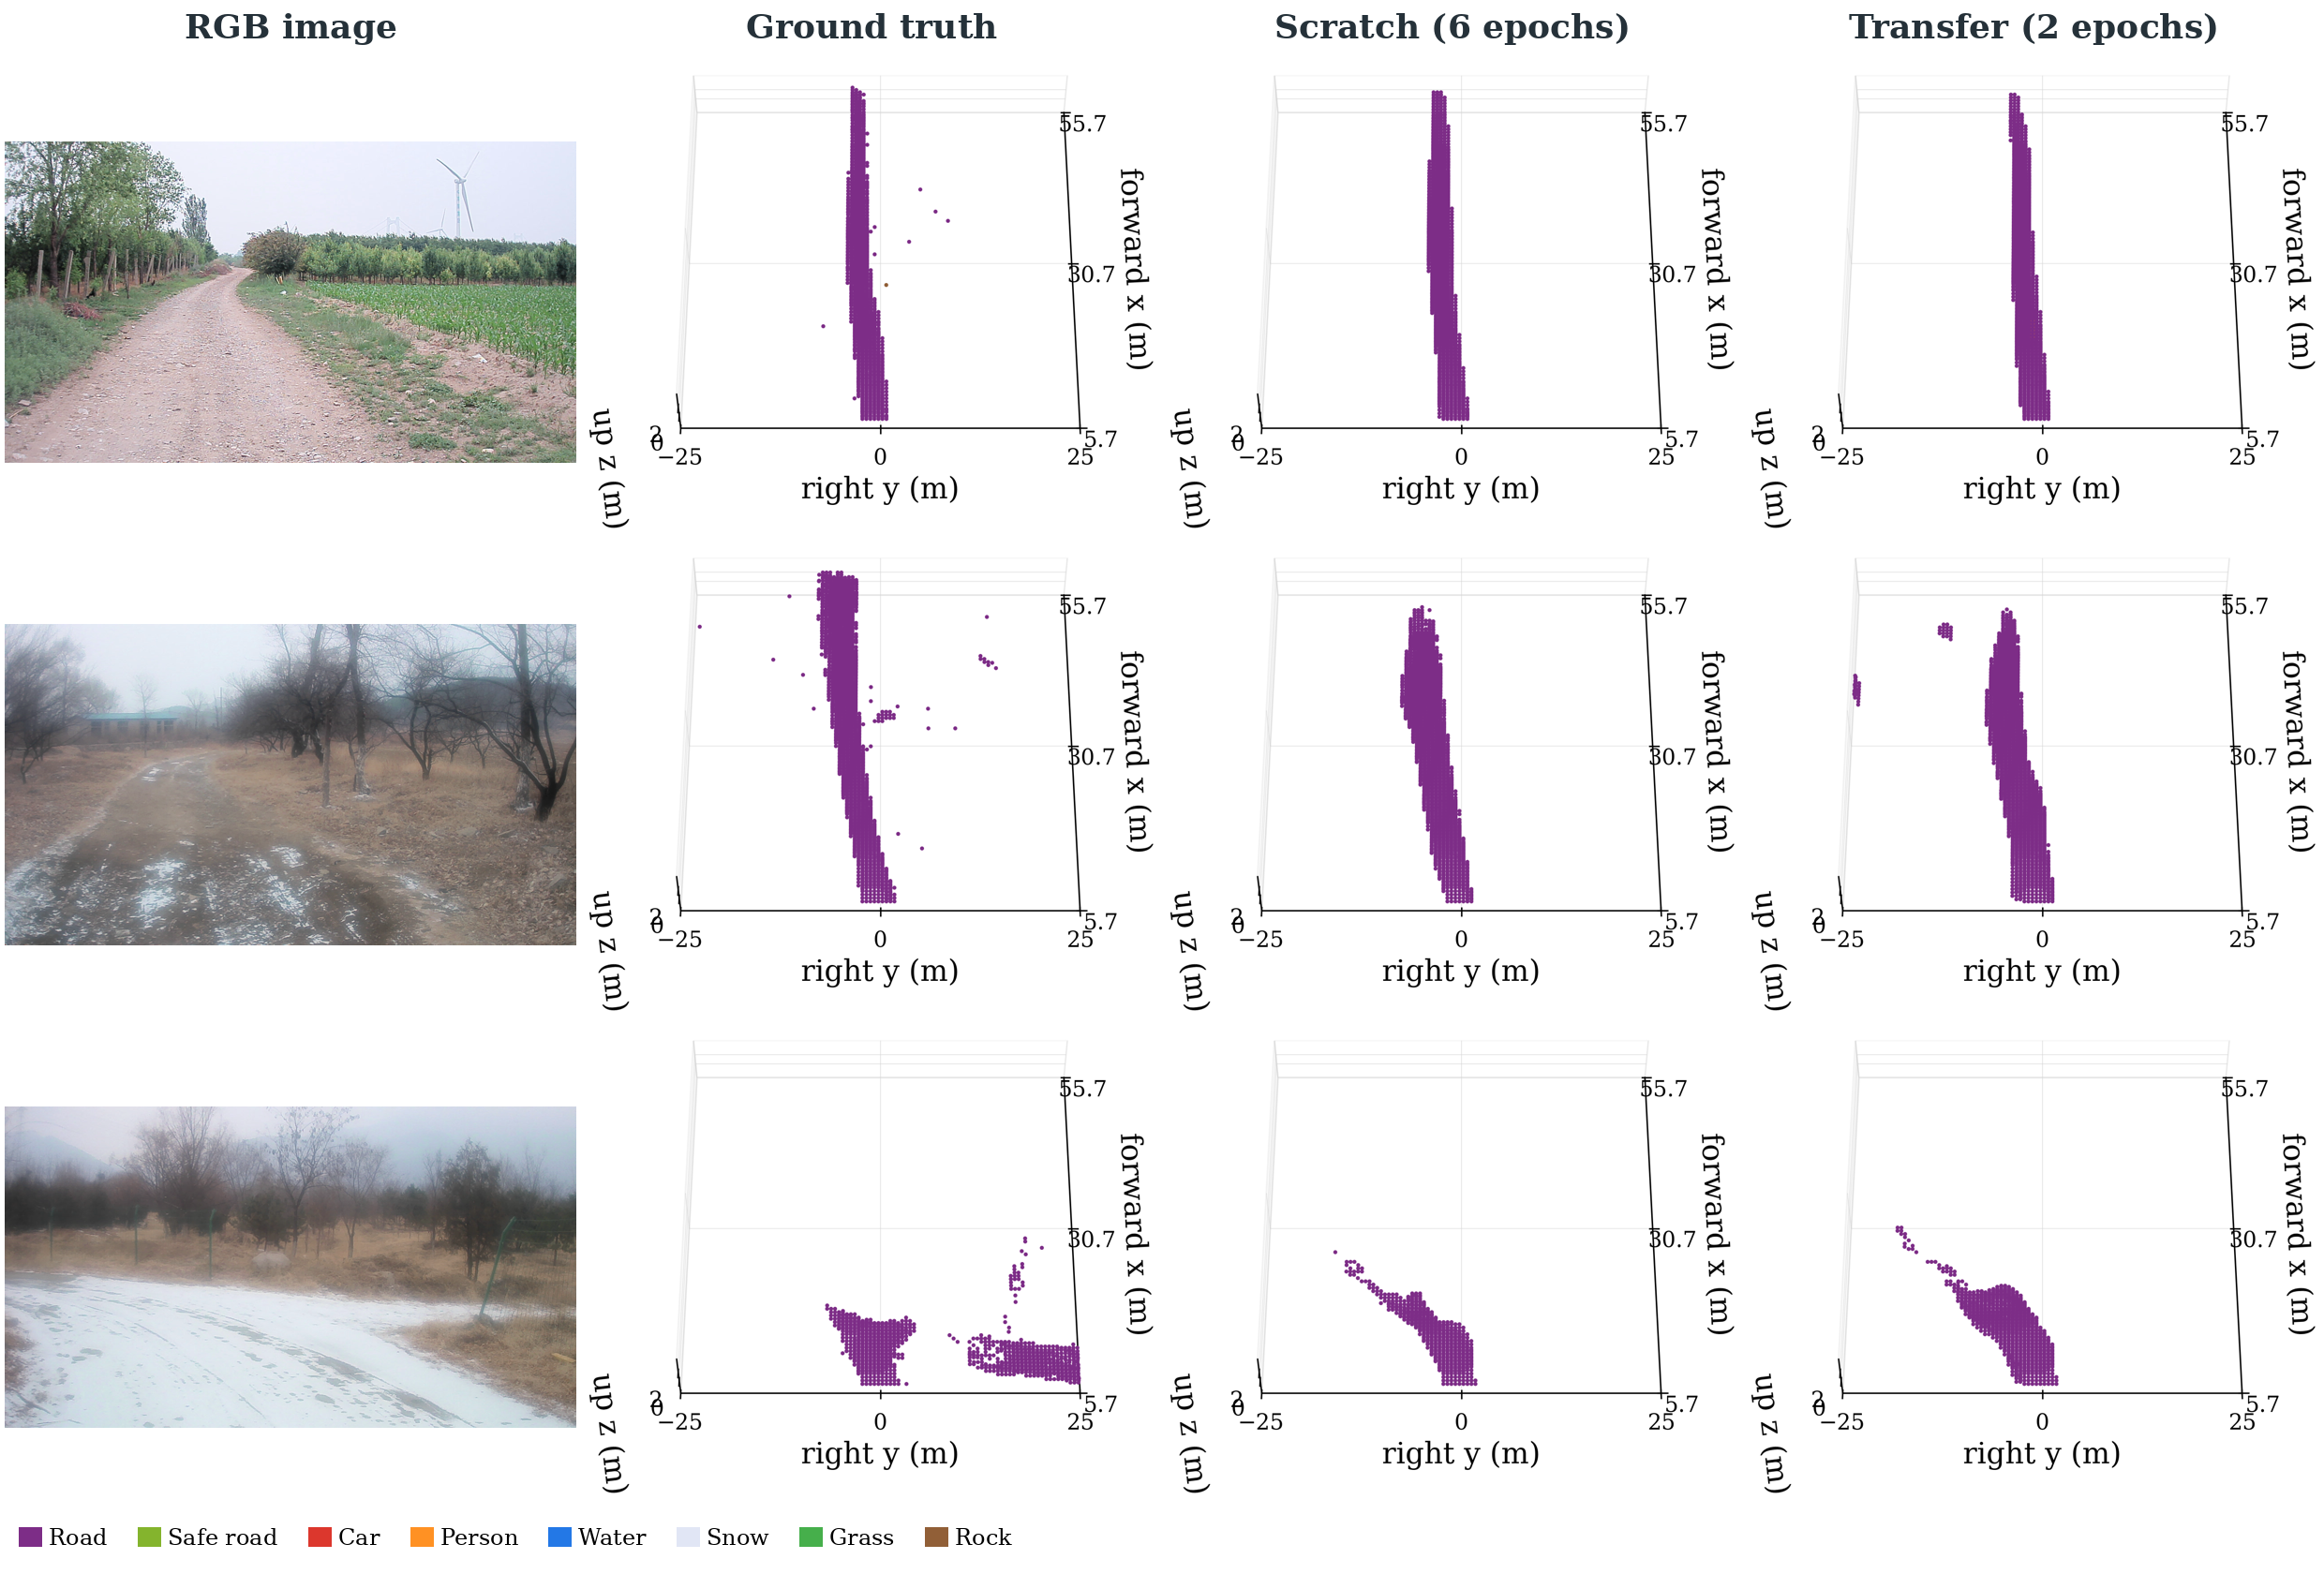
\includegraphics[width=\linewidth]{orad_transfer.png}
\caption{Qualitative transfer results on ORAD-3D. Columns show monocular RGB, GT, training from scratch, and transfer from the source domain. Both models use the official target-domain grid and the same viewpoint above and directly behind the mobile platform; free space is hidden.}
\label{fig:orad}
\end{figure}

\subsection{Voxel-resolution transfer}\label{sec:resolution}
AgriOcc-Dataset uses a voxel resolution of $0.2\,\mathrm{m}$, consistent with mainstream autonomous-driving semantic occupancy benchmarks~\citep{behley2019semantickitti,li2024sscbench}.
For agricultural mobile platforms traveling between ridges, avoiding obstacles between plants, or performing precision operations, however, $0.2\times0.2\times0.2\,\mathrm{m}$ voxels may quantize neighboring crops, narrow furrows, or local drivable-area boundaries into the same cell, potentially limiting accuracy.
Directly extending the entire BEV encoder to $0.1\times0.1\times0.2\,\mathrm{m}$ increases the number of XY queries fourfold, from $75\times75$ to $150\times150$.
This substantially increases computation and memory costs for multi-scale image--BEV interactions, intermediate BEV activations, and 3D occupancy supervision.
We therefore collect an additional small simulation dataset at $0.1\times0.1\times0.2\,\mathrm{m}$ resolution, containing 19,300 samples split equally into training and validation sets.
We use it to further investigate whether AgriOcc can efficiently transfer its learned standard-resolution 3D priors to finer-resolution occupancy prediction.

The transfer model is first trained on AgriOcc-Dataset at $0.2\times0.2\times0.2\,\mathrm{m}$ resolution.
On the $0.1\times0.1\times0.2\,\mathrm{m}$ data, we compare two adaptation approaches with a frozen backbone.
\emph{Query adaptation} retains the backbone parameters and learns only the $150\times150$ high-resolution BEV query grid.
\emph{Refinement-head adaptation} retains the original $75\times75$ BEV encoder and Agri-AMoE decoder, freezes all existing weights, and trains only a learnable $2\times$ refinement head at the occupancy output.
This head fuses coarse occupancy logits with a projection of the corresponding BEV features and outputs $150\times150\times25$ voxels.
The control model does not use the $0.2\,\mathrm{m}$ occupancy-pretrained weights, instead learning high-resolution $150\times150$ BEV representations and occupancy prediction from scratch on the same $0.1\,\mathrm{m}$ dataset.
All three configurations are trained for 15 epochs using the same small spatial region and high-resolution labels. Measured results are reported in Table~\ref{tab:resolution}.

\begin{table}[pos=htbp]
\centering
\caption{Voxel-resolution transfer. IoUs are reported in \%, and time denotes logged wall-clock hours for 15 epochs of target-resolution training and per-epoch validation, excluding source training at $0.2\,\mathrm{m}$. All configurations output $150\times150\times25$ voxels.}
\label{tab:resolution}
\resizebox{\linewidth}{!}{%
\begin{tabular}{lrrrrrrrr}
\toprule
Setting & Time (h) & mIoU & Free & Crop & Soil & Drivable & Other veg. & Other obs.\\
\midrule
0.1 m from scratch & 15.47 & 46.55 & 92.27 & 22.42 & 66.66 & 39.51 & 33.44 & 25.00 \\
Query adaptation (frozen backbone) & 11.40 & 45.34 & 91.67 & 22.43 & 64.72 & 30.70 & 34.82 & 27.71 \\
Refinement-head adaptation (frozen backbone) & 4.72 & 49.67 & 92.70 & 29.10 & 71.72 & 38.51 & 36.84 & 29.14 \\

\bottomrule
\end{tabular}}
\end{table}

As shown in Table~\ref{tab:resolution}, refinement-head adaptation achieves 49.67\% mIoU, exceeding the 46.55\% obtained by training from scratch without $0.2\,\mathrm{m}$ occupancy pretraining by 3.12 percentage points. Crop IoU increases from 22.42\% to 29.10\%.
Training time decreases from 15.47 to 4.72 hours, a reduction of 69.5\%. It also achieves the best IoU in five semantic classes.
Although query adaptation reduces training time to 11.40 hours, its mIoU of 45.34\% does not exceed training from scratch.
The refinement head reuses the scene layout and semantic relationships already established by the low-resolution network, using the limited target data to learn local residuals at the output. Query adaptation instead changes the spatial sampling density of all BEV queries and must still reconcile fine-grid representations with a frozen backbone.
Refinement-head adaptation preserves the stable global context of the $75\times75$ encoder and uses only 11,238 trainable parameters to learn high-frequency residuals from coarse 0.2 m predictions to 0.1 m voxels.
High-resolution supervision can thus focus on recovering inter-plant boundaries, furrows, and local drivable areas, without relearning camera projection relationships and scene-level semantic layouts.
These results demonstrate that a frozen backbone and a lightweight refinement head can effectively transfer AgriOcc trained on $0.2\,\mathrm{m}$ data to higher-resolution occupancy prediction, achieving higher accuracy than training from scratch with substantially shorter adaptation time.

\subsection{From semantic occupancy to crop-row fitting}\label{sec:crop_row_fitting}
To examine whether occupancy representations provide row-level geometric information, we conduct offline crop-row fitting experiments on separately collected field-driving sequences.
The evaluation set contains 64 sequences and 1,540 frames covering nine crops. Geometric row segments provided by the planting layout serve as ground truth.

\paragraph{Shared post-processing from occupancy to row lines}
We separately project Crop voxels from semantic occupancy labels and model predictions along the height dimension to form BEV density maps, extract candidate rows through orientation search, and fit straight lines using RANSAC and weighted least squares.
The midline between the adjacent crop rows flanking the vehicle is then taken over their common support interval to obtain a navigation centerline for each frame.

\paragraph{Navigation-line error evaluation}
We use the centerline between the adjacent valid planting rows flanking the vehicle, exported by the simulation system, as ground truth and evaluate navigation-centerline fitting using lateral root mean squared error (RMSE).
We compare fitting results from semantic occupancy labels and predictions of the trained semantic occupancy model.
To ensure comparability, we evaluate only frames in which the ground-truth, label-derived, and prediction-derived centerlines share at least $2\,\mathrm{m}$ of longitudinal support. All centerlines are sampled at identical forward positions with spacing no greater than $0.05\,\mathrm{m}$, including both interval endpoints.
Let $\mathcal F$ denote the set of jointly valid frames and $N_f$ the number of sample points in frame $f$. Then,

\begin{equation}
 \operatorname{RMSE}_s=\sqrt{\frac{
 \sum_{f\in\mathcal F}\sum_{k=1}^{N_f}
 \left[y_{s,f}(x_{f,k})-y_{g,f}(x_{f,k})\right]^2}{
 \sum_{f\in\mathcal F}N_f}},\qquad s\in\{\mathrm{label},\mathrm{pred}\}.
\end{equation}
where $y_{g,f}$ is the geometric reference centerline and $y_{s,f}$ is the centerline fitted from the corresponding occupancy result, measured in m.
We additionally report mean absolute error (MAE), computed by averaging the absolute lateral deviations between fitted and geometric reference centerlines over the same valid sample points, also in m.
MAE measures the mean distance of the centerline from the reference position, with lower values indicating better performance. Compared with RMSE, it is less sensitive to a small number of large deviations.

\begin{table}[pos=htbp]
\centering
\caption{Errors of the navigation centerline between crop rows. Lower RMSE and MAE are better.}
\label{tab:crop_centerline_rmse}
\begin{tabular*}{\linewidth}{@{\extracolsep{\fill}}lrrr}
\toprule
Centerline source & Lateral RMSE & Lateral MAE \\
\midrule
Semantic occupancy labels & 0.201 & 0.143 \\
AgriOcc occupancy predictions & 0.309 & 0.212 \\

\bottomrule
\end{tabular*}
\end{table}

Table~\ref{tab:crop_centerline_rmse} reports navigation-centerline errors for the two occupancy sources.
On the same frames and sample points, the lateral RMSE values for label-derived and prediction-derived occupancy centerlines are 0.201 m and 0.309 m, respectively.
Both sets of errors include the effects of row fitting and the choice of the inter-row passage, while the prediction-derived results are additionally affected by semantic occupancy prediction errors.

Figure~\ref{fig:crop_row_3d_rgb} shows RGB images and fitting results from semantic occupancy labels and predictions for carrot, corn, and tomato samples.
The 3D views overlay crop-row lines and inter-row navigation centerlines on the occupancy maps, illustrating the row-level geometric information provided by occupancy representations.

\begin{figure}[pos=htbp]
\centering
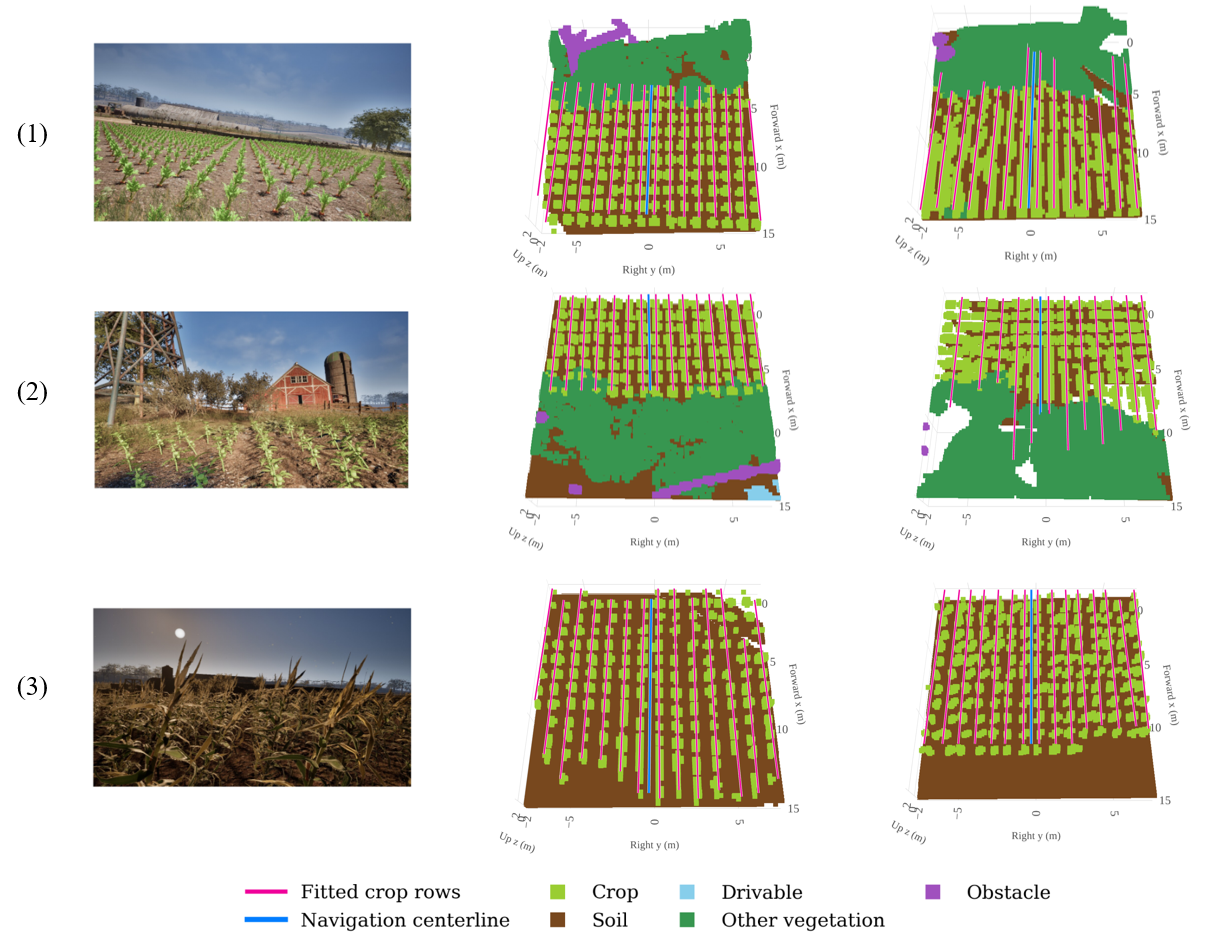
\includegraphics[width=\linewidth]{crop_row_3d_rgb.png}
\caption{3D visualization of crop-row fitting and navigation centerlines. The three columns show the current forward-facing RGB image, fitting results from semantic occupancy labels, and fitting results from AgriOcc occupancy predictions. Magenta lines denote fitted crop rows, and blue lines denote navigation centerlines between adjacent crop rows. All occupancy views share the same viewpoint, coordinate range, and semantic colors. For visibility, the overlaid lines are displayed above the crop canopy. The blue centerlines serve as inter-row geometric references and have not undergone traversability checks.}
\label{fig:crop_row_3d_rgb}
\end{figure}

\subsection{Discussion and limitations}\label{sec:discussion}
The proposed semantic occupancy prediction model perceives surrounding spatial structures and common elements in agricultural scenes, supporting applications such as road recognition, crop-row recognition, obstacle perception, and obstacle avoidance for agricultural mobile platforms.
However, the current work provides semantic predictions without instance-level perception. For dynamic obstacles such as moving vehicles, agricultural machinery, or animals, it cannot determine the object instance to which a group of voxels belongs.
Local path planning based on the motion trends of surrounding objects therefore requires an additional object detection model.
AgriOcc is consequently better suited to agricultural scenes with few moving objects.
In future work, we will investigate panoptic instance-level semantic occupancy for agricultural mobile platforms to improve their perception in complex environments.

\section{Conclusion and Future Work}\label{sec:conclusion}
This work addresses 3D environmental perception for agricultural mobile platforms through the AgriOcc semantic occupancy framework and a simulation dataset covering ten crops, multiple growth stages, times of day, and weather conditions.
AgriOcc retains BEVFormer's deformable BEV aggregation architecture, uses Agri-AMoE to model anisotropy in ground structures, plant heights, and local context, and increases exposure to crop supervision through crop-aware sampling while keeping the training length fixed.
Over a $15\times15\times5\,\mathrm{m}$ prediction region ahead of the mobile platform, the model achieves 64.08\% mIoU and 39.38\% crop IoU.
Ablation experiments reveal distinct roles for structure-adaptive decoding and exposure to crop samples: the former improves the underlying representation, while the latter further adjusts the decision balance between crops and background.
Resolution-transfer experiments show that retaining a stable coarse-scale model and training only a lightweight refinement head can transfer $0.2\,\mathrm{m}$ occupancy priors to $0.1\times0.1\times0.2\,\mathrm{m}$ outputs, improving accuracy while reducing training time at the target resolution.
Real-world transfer experiments further show that AgriOcc trained on simulation data can learn environmental features applicable to the real world.

Future work will develop richer cross-domain training strategies for variations in real farmland illumination, weather, crop growth stages, and sensor perturbations; investigate panoptic instance-level semantic occupancy for agricultural mobile platforms to improve dynamic perception; and closely integrate AgriOcc's occupancy representations with risk-aware traversability analysis, trajectory optimization, and closed-loop navigation.
Ultimately, semantic occupancy may provide a stable 3D foundation-model interface connecting perception, decision-making, and control across agricultural mobile platforms.

\section*{Acknowledgement}
This work was supported by the Natural Science Foundation of China [Grant No. 12373107].

\section*{CRediT Authorship Contribution Statement}
Lei He: Conceptualization, methodology, software, data curation, formal analysis, investigation, visualization, and writing---original draft. 
Jing Jin: Conceptualization, methodology, supervision, project administration, funding acquisition, and writing---review and editing. 
Yi Liu: Methodology, validation, formal analysis, and writing---review and editing.

\section*{Data and code availability}
The construction pipeline, class definitions, and annotation-generation procedure of AgriOcc-Dataset are described in Section~\ref{sec:dataset_construction}.
The dataset and code used in this study are planned for public release for non-commercial research after the paper is accepted.

\section*{Declaration of competing interests}
The authors declare no competing interests that could have influenced the work reported in this paper.



\bibliographystyle{cas-model2-names}
\bibliography{references}
\end{document}
